\documentclass[10pt,a4paper,draft]{article}
%\documentclass[10pt,a4paper]{article}

%\usepackage[top=3cm, bottom=0cm, left=3.5cm,right=2cm]{geometry}
\usepackage[top=1in, left=1in ,right=1in, bottom=1in, footskip=0in, marginparwidth=0in]{geometry}

% use Unicode characters - try changing the option if you run into troubles with special characters (e.g. umlauts)
\usepackage[utf8]{inputenc}

\usepackage{fancyhdr}

% clean citations
%\usepackage{cite}
%\usepackage[super,sort&compress,comma]{natbib}
\usepackage[numbers, round, sort&compress, comma]{natbib}
%\usepackage[round]{natbib}

% hyperref makes references clicky. use \url{www.example.com} or \href{www.example.com}{description} to add a clicky url
%\usepackage{nameref,hyperref}

% math
\usepackage{amsmath,amsfonts,amssymb}
\usepackage{bbold}

% line numbers
\usepackage[right]{lineno}

% improves typesetting in LaTeX
\usepackage{microtype}
\DisableLigatures[f]{encoding = *, family = * }
\usepackage{enumitem}

% text layout - change as needed
%\raggedright
%\setlength{\parindent}{0.5cm}
%\textwidth 5.25in 
%\textheight 8.75in

% Remove % for double line spacing
%\usepackage{setspace} 
%\doublespacing

% adjust caption style
\usepackage[aboveskip=1pt,labelfont=bf,labelsep=period,singlelinecheck=off]{caption}

% remove brackets from references
\makeatletter
\renewcommand{\@biblabel}[1]{\quad#1.}
\makeatother

% use \textcolor{color}{text} for colored text (e.g. highlight to-do areas)
\usepackage{color}

% define custom colors (this one is for figure captions)
\definecolor{Gray}{gray}{.25}

% this is required to include graphics
\usepackage{graphicx}
\usepackage{sidecap}

% hyperlinks
\usepackage{hyperref}

% change name of Table of contents
\renewcommand*\contentsname{Supporting Information}

% ########################################################

%\pagestyle{headings}
\pagestyle{myheadings}
\markright{}

\hyphenation{math-e-mat-i-cal-ly} 
\hyphenation{inter-neurons} 

\begin{document}

\thispagestyle{empty}

% title goes here:
\begin{flushleft}
{\Large
\textbf\newline{Title}
}
%\newline
%% authors go here:
%\\
%Loreen Hert\"ag\textsuperscript{1,*},
%Claudia Clopath\textsuperscript{1,§}
%\\
%\bigskip
%\bf{1} Bioengineering Department, Imperial College London, London, UK.
%\\
%\bigskip
%* l.hertag@imperial.ac.uk, § c.clopath@imperial.ac.uk

\end{flushleft}

% now start line numbers
%\linenumbers

\begin{abstract}
blahhh blahhh blah
\end{abstract}

\section*{Introduction}
%
To survive in an ever-changing environment, animals must flexibly adapt their behavior based on previously encoded and novel information. This context-dependency must also be reflected in the information processing of neural networks underlying intelligent behavior. For instance, when you walk down some staircase in your fully lit basement, your brain might entirely rely on the feedforward (bottom-up) input your senses receive (Fig. \ref{fig:Fig_1}, left). In contrast, when you walk down the same stairs in complete darkness, your brain might rely entirely on feedback (top-down) signals generated from a staircase model it has formed over previous experiences (Fig. \ref{fig:Fig_1}, middle). 

The importance of these feedback inputs has been emphasized by observations showing that top-down projections outnumber feedforward connections (XXX) and that they modulate (XXX) or even entirely drive (XXX) neuron activity. But how do neural networks switch between a feedforward-dominated and a feedback-dominated processing mode? And how do neural networks combine both input streams wisely? For instance, if you hike down an unexplored mountain in very foggy conditions, your brain receives unreliable visual information. In addition, it can only draw on a shaky prediction about what to expect (Fig. \ref{fig:Fig_1}, right). 

A common hypothesis is that the brain weights different inputs according to their reliabilities. A prominent example of this hypothesis is Bayesian multisensory integration (XXX). According to this theory, neural networks represent information from multiple modalities by a linear combination of the uncertainty-weighted single-modality estimates. Multisensory integration is supported by several observations showing that xxx (XXX). It is conceivable that the same concepts can be employed for the weighting of sensory inputs and predictions thereof (XXX). A central point in the weighting of inputs is the estimation of variances as a measure of uncertainty. However, how the variance of both the sensory input and the prediction can be computed on the circuit level is not resolved yet.  

We hypothesised that prediction error (PE) neurons provide the basis for the neural computation of variances. PEs are an integral part of the theory of predictive processing which states that the brain constantly compares incoming sensory information with predictions. When those predictions are wrong, the resulting PEs allow the network to revise the model of the world, thereby ensuring that the predictions are more accurate (XXX). Experimental evidence suggests that these PEs may be represented in the activity of distinct groups of neurons, termed PE neurons (XXX). Moreover, these neurons may come in two types when excitatory neurons exhibit near-zero, spontaneous firing rates (XXX). Negative PE (nPE) neurons mainly increase their activity when the prediction is \textit{stronger} than the sensory input, while positive PE (pPE) neurons mainly increase their activity when the prediction is \textit{weaker} than the sensory input. Indeed, it has been shown that excitatory neurons in layer 2/3 of rodent primary sensory areas can encode negative or positive PEs (XXX). 

Here, we show that the unique response patterns of nPE and pPE neurons may provide the backbone for computing both the mean and the variance of sensory stimuli. Furthermore, we suggest a network model with a hierarchy of PE circuits to estimate the variance of the prediction, in addition to the variance of the sensory inputs. In line with multisensory integration, predictions are weighted more strongly than the sensory stimuli when the environment is stable (that is, predictable) but the sensory inputs are noisy. Moreover, we show that predictions are integrated more strongly after a change in the environment, even when the new sensory stimulus is reliable. In addition, we unravel the mechanisms underlying a neuromodulator-induced shift in the weighting of sensory inputs and predictions. In our model, these neuromodulators activate groups of inhibitory neurons like parvalbumin-expressing (PV), somatostatin-expressing (SOM), and vasoactive intestinal peptide-expressing (VIP) interneurons (XXX). In a computational model, these interneurons have been shown to establish a multi-pathway balance of excitation and inhibition that is the basis for nPE and pPE neurons (XXX). By breaking this balance, the excitatory neurons change their baseline firing rate and gain, leading to a biased variance estimation. Finally, we show that this weighting can be understood as the neural manifestation of the contraction bias (XXX). 

%
\begin{figure}[t!]
	\centering
    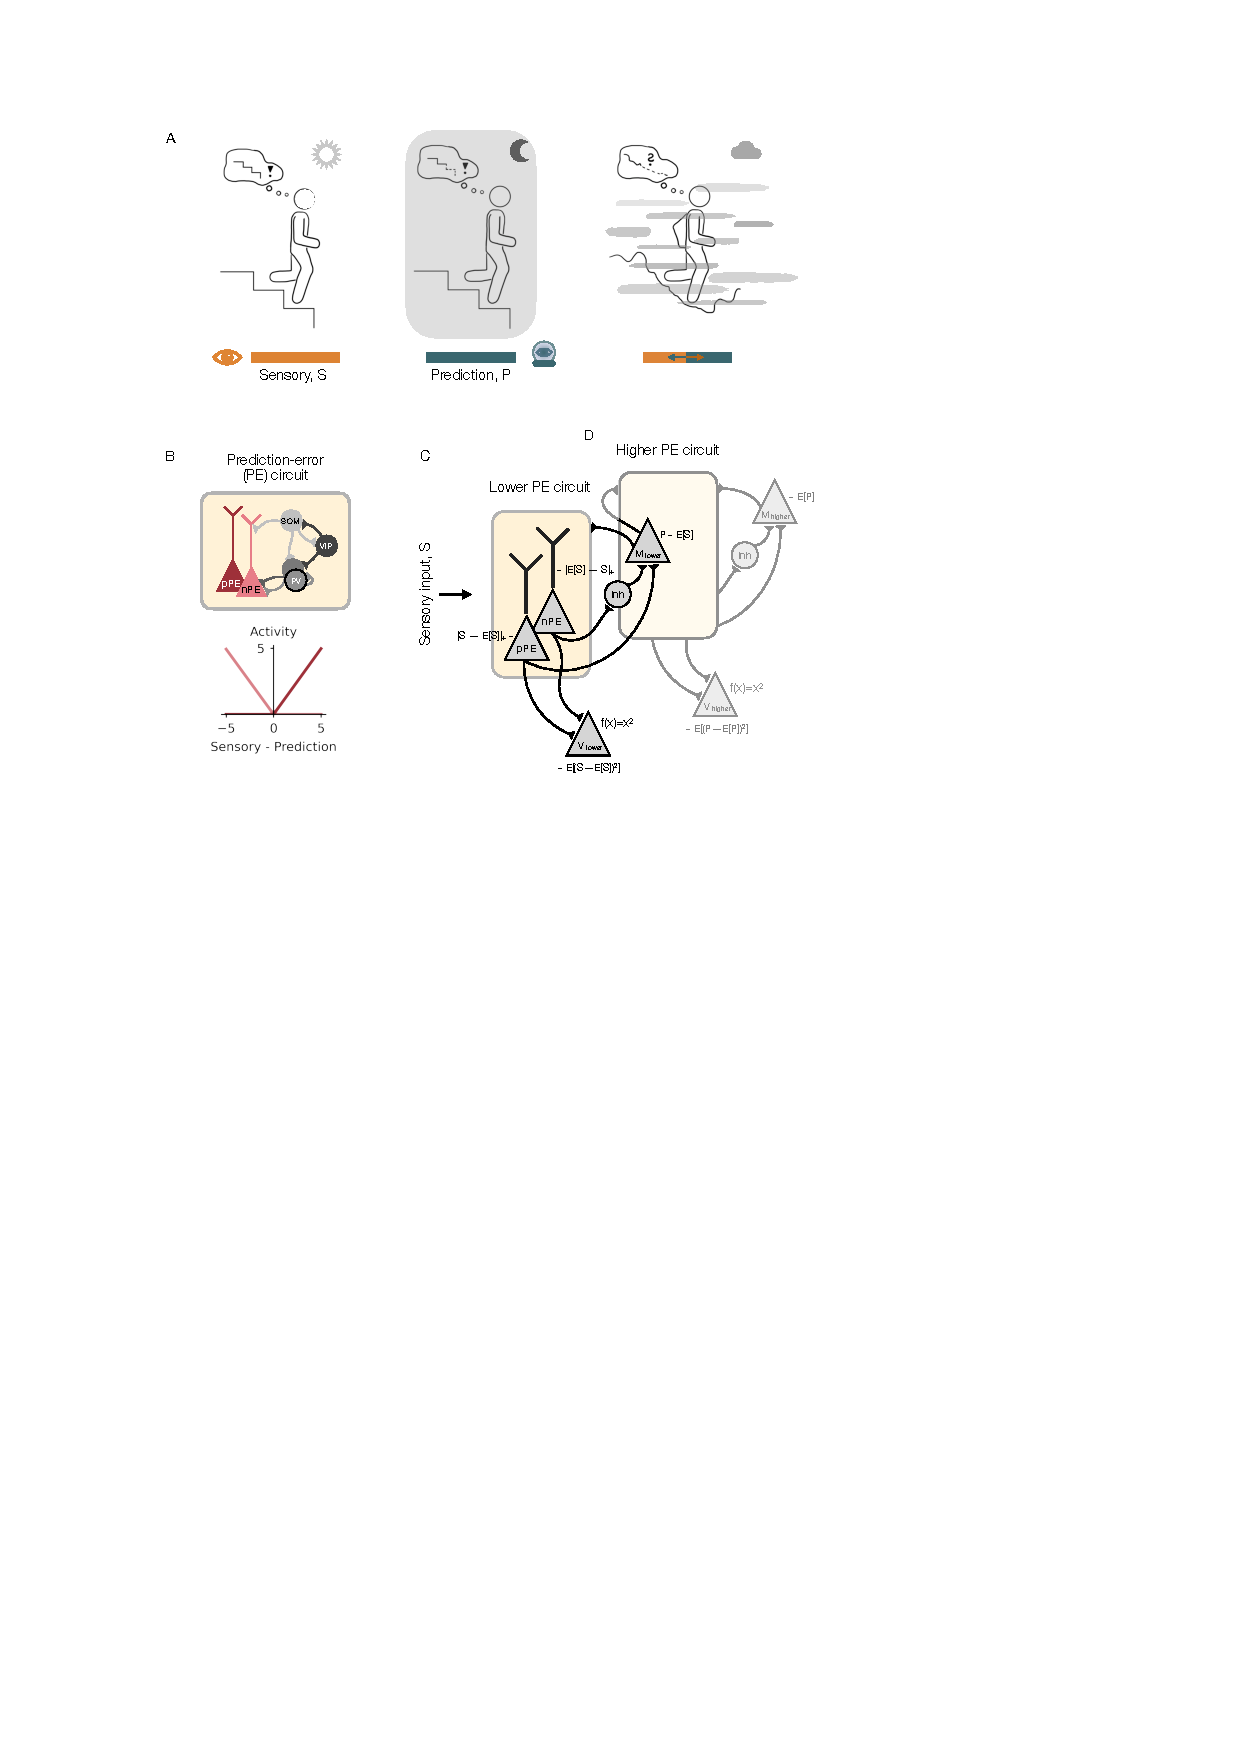
\includegraphics{../results/figures/final/Fig_1}
\caption{\footnotesize{\bf Neural network model to flexibly integrate sensory information and predictions.\newline} 
{\bf (A)} Example illustration of context-dependent integration of information. Left: When walking down a staircase that is clearly visible, the brain might rely solely on external sensory information. Middle: When walking down the same stairs in the absence of visual information, the brain might rely on predictions formed by previous experience. Right: When climbing down an unexplored mountain in foggy conditions, the brain might need to integrate sensory information and predictions at the same time.
{\bf (B)} Illustration of a prediction-error (PE) circuit with both negative and positive PE (nPE/pPE) neurons that receive inhibition from three different inhibitory interneuron types: parvalbumin-expressing (PV), somatostatin-expressing (SOM), and vasoactive intestinal peptide-expressing (VIP) interneurons. Local excitatory connections are not shown for clarity.
{\bf (C)} Illustration of network model that estimates the mean and variance of the external sensory stimuli. The core of this network model is the PE circuit shown in (B). The lower-level V neuron encodes the variance, while the lower-level M neuron encodes the mean of the sensory input.
{\bf (D)} Same as in (C) but the feedforward input is the activity of the lower-level M neuron.
}
\label{fig:Fig_1}
\end{figure}
%


\section*{Results}
%

\subsection*{nPE and pPE neurons as the basis for estimating mean and variance of sensory stimuli}
%
We hypothesise that the distinct response patterns of negative and positive prediction-error (nPE/pPE) neurons represent the backbone for estimating the mean and the variance of sensory stimuli. nPE neurons only increase their activity relative to a baseline when the sensory input is weaker than predicted, while pPE neurons only increase their activity relative to a baseline when the sensory input is stronger than predicted. Moreover, both nPE and pPE neurons remain at their baseline activity when the sensory input is fully predicted (XXX). Assuming that the prediction equals the mean of the sensory stimulus, the PE neurons, hence, encode the deviation from the mean. Thus, the squared sum of nPE and pPE neuron activity represents the variance of the feedforward input. 
%
\begin{figure}[t!]
	\centering
	%\makebox[\textwidth][c]{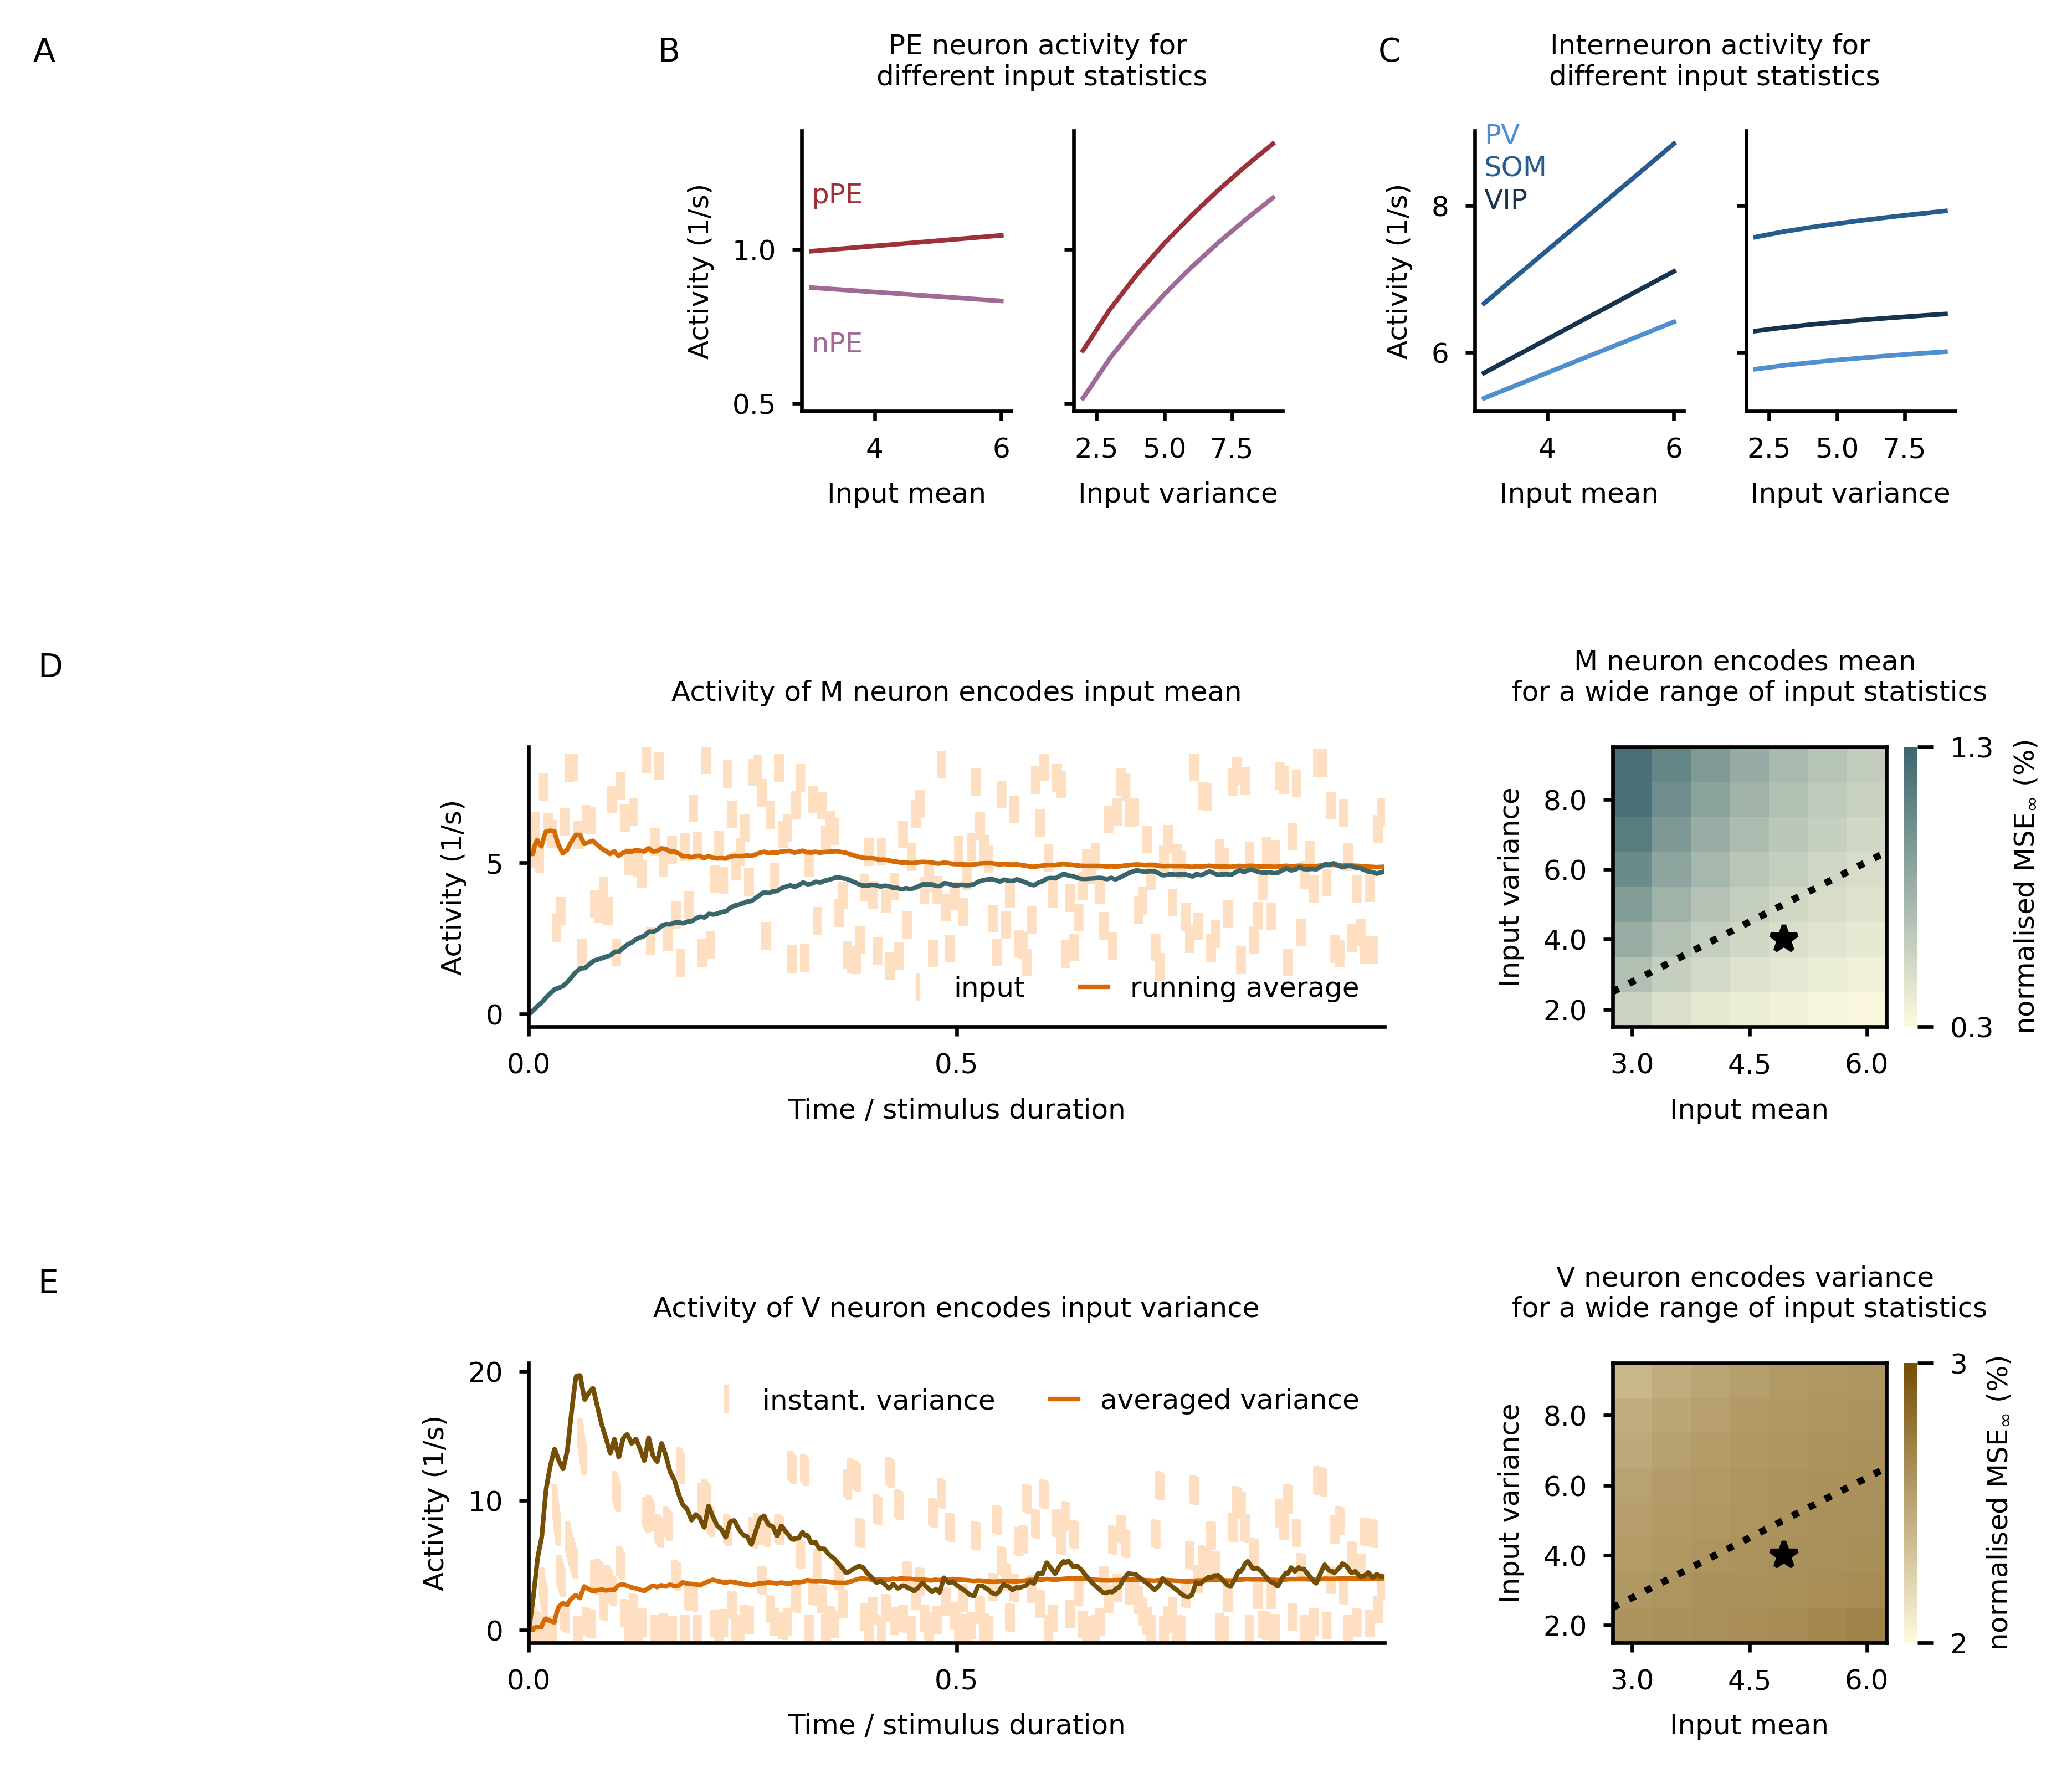
\includegraphics{../results/figures/final/Fig_2}}
    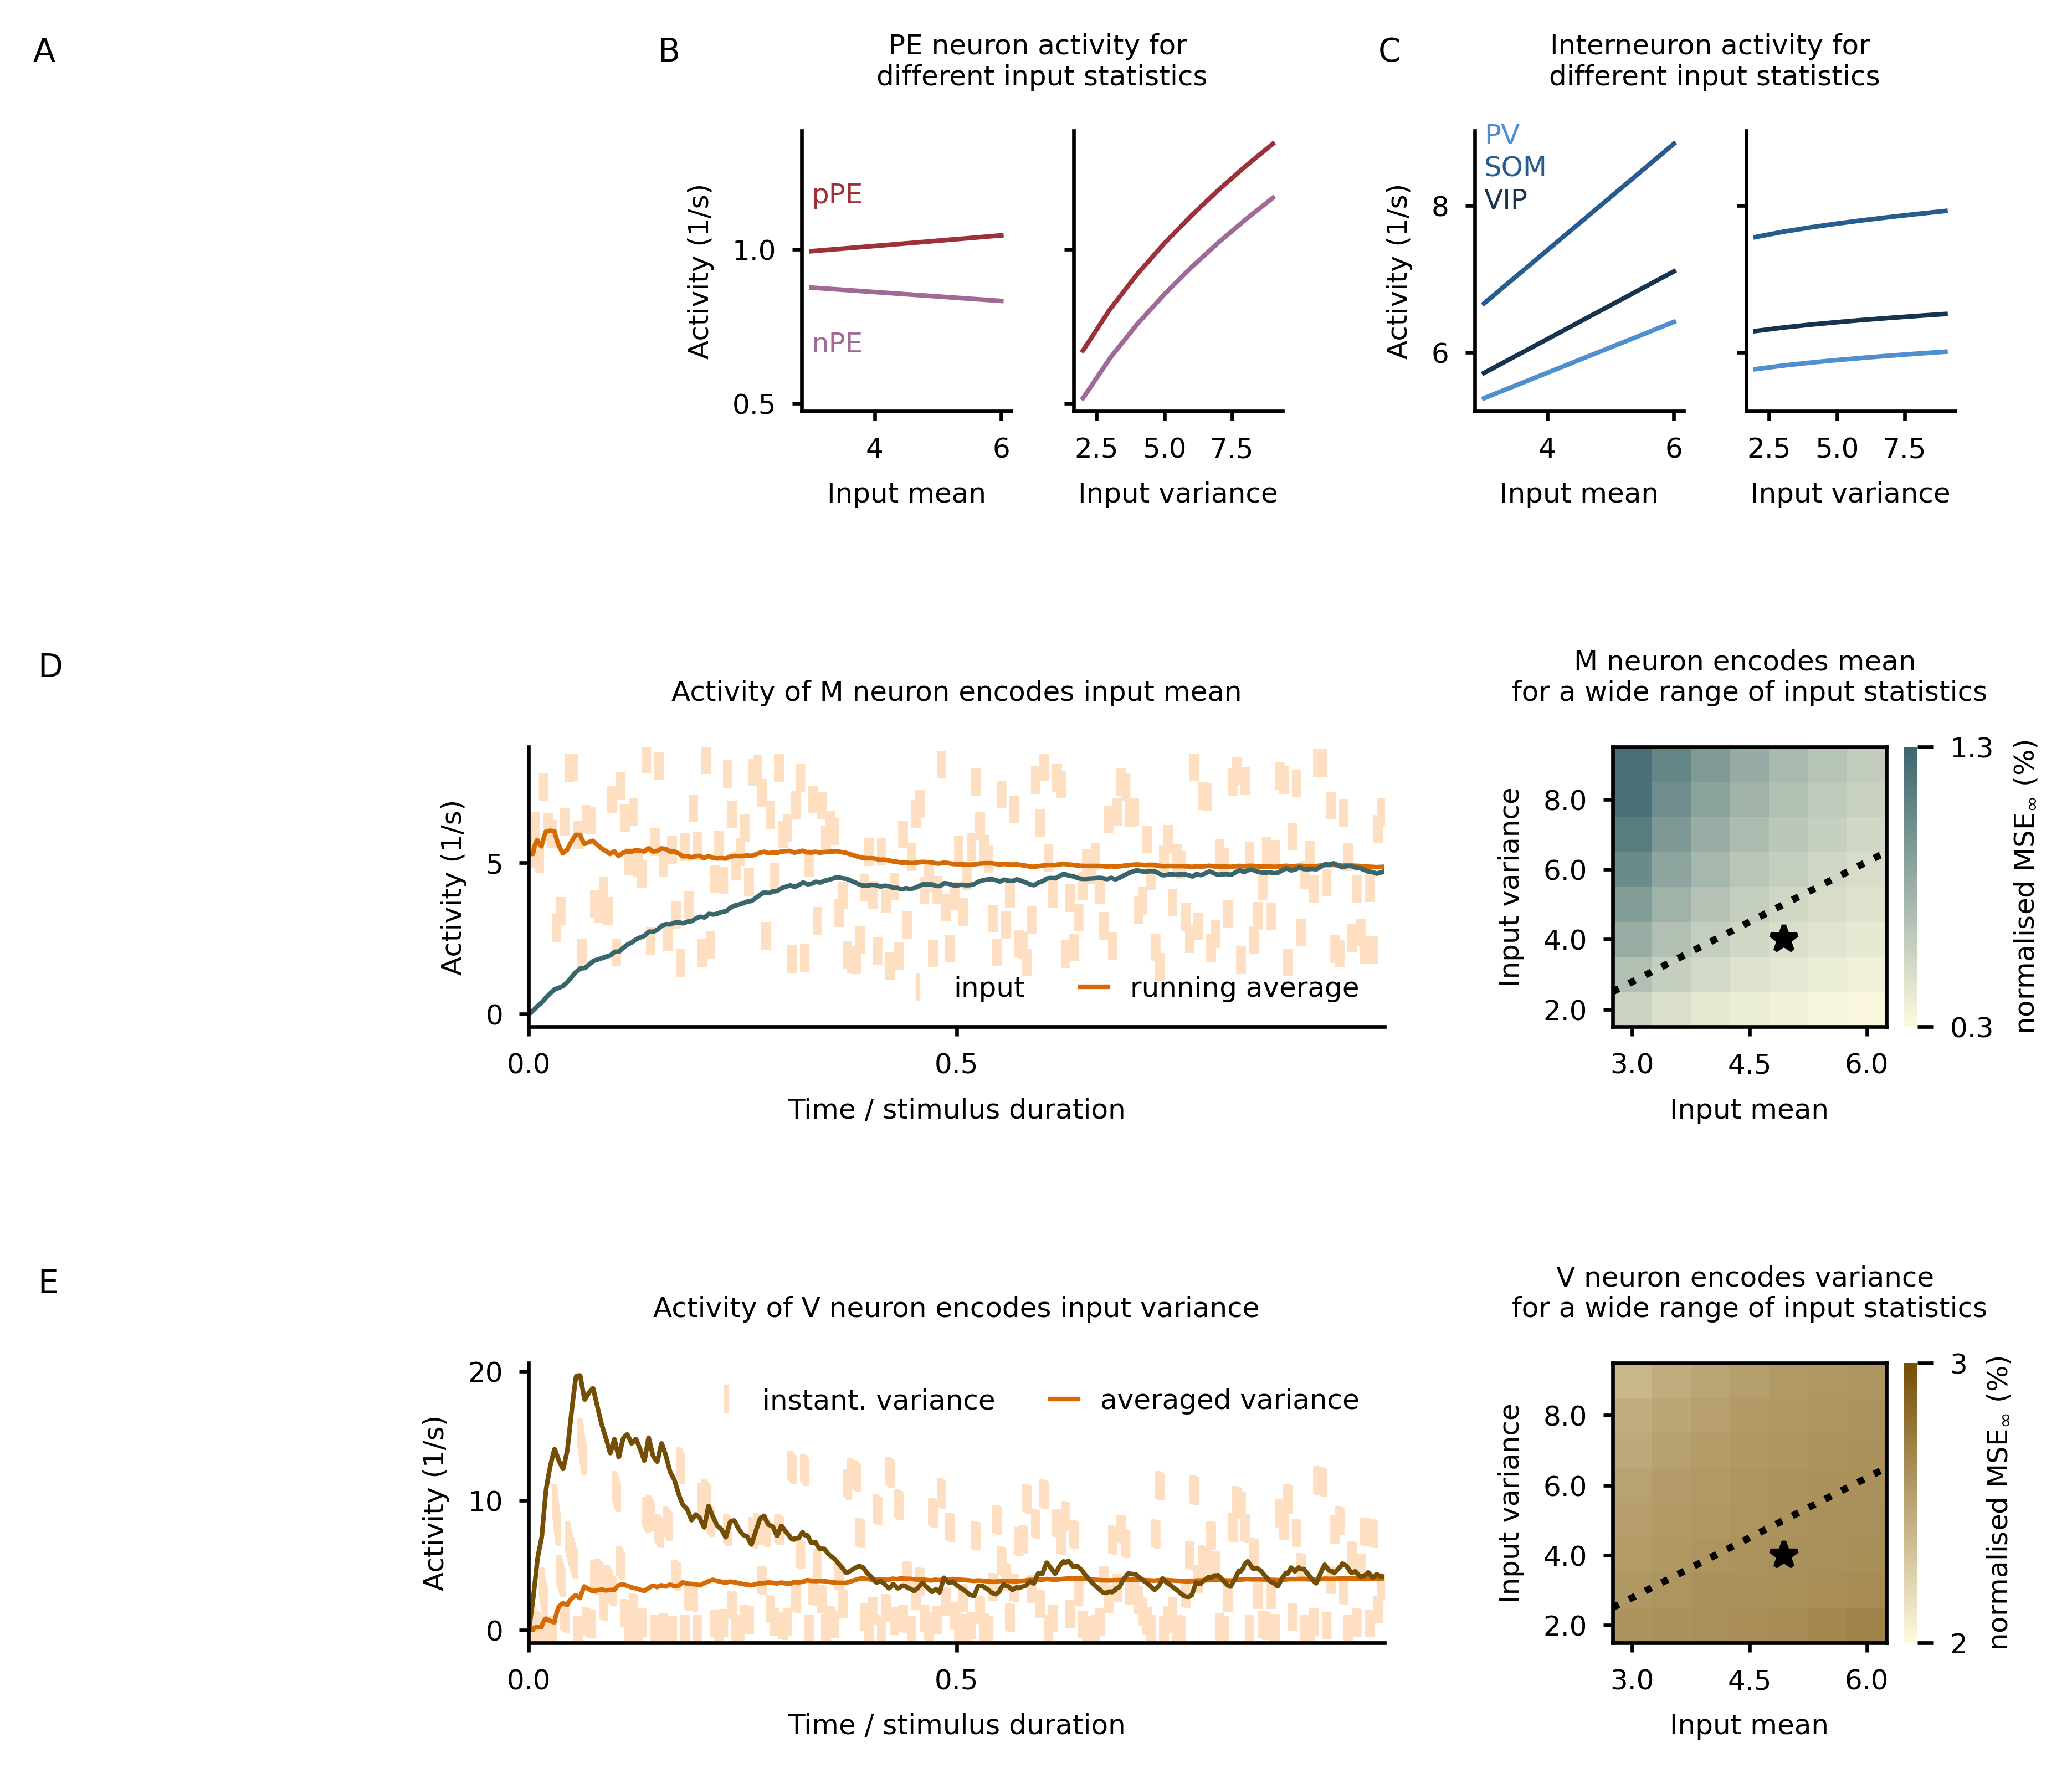
\includegraphics[width=1\linewidth]{../results/figures/final/Fig_2}
\caption{\footnotesize{\bf Prediction-error neurons provide the basis for estimating mean and variance of sensory stimuli.\newline} 
{\bf (A)} Illustration of the inputs with which the network shown in \ref{fig:Fig_1}C is stimulated. Network is exposed to a sequence of constant stimuli drawn from a uniform distribution. Stimulus duration is XXX.
{\bf (B)} PE neuron activity hardly changes with stimulus strength (left) but strongly increases with stimulus variability (right).
{\bf (C)} Interneuron activity strongly changes with stimulus strength (left) but hardly changes with stimulus variability (right) .
{\bf (D)} M neuron correctly encodes the mean of the sensory stimuli. Left: Illustration of the input synapses onto the M neuron. Middle: Activity of the M neuron over time for a uniform distribution with mean XXX and standard deviation XXX. Right: Normalised mean-squared error (MSE) between the running average and the M neuron activity for different parametrizations of the stimulus distribution.
{\bf (E)} V neuron correctly encodes the variance of the sensory stimuli. Left: Illustration of the input synapses onto the V neuron. Middle: Activity of the V neuron over time for a uniform distribution with mean XXX and standard deviation XXX. Right: Normalised mean-squared error (MSE) between the instantaneous variance and the V neuron activity for different parametrizations of the stimulus distribution.
}
\label{fig:Fig_2}
\end{figure}
%

To test our hypothesis, we studied a rate-based mean-field network the core of which is a prediction-error (PE) circuit with excitatory nPE and pPE neurons, as well as inhibitory parvalbumin-expressing (PV), somatostatin-expressing (SOM), and vasoactive intestinal peptide-expressing (VIP) interneurons (Fig. \ref{fig:Fig_1}B). While the excitatory neurons are simulated as two coupled point compartments to emulate the soma and dendrites of elongated pyramidal cells, respectively, all inhibitory cell types were modeled as point neurons. The connectivity of and inputs to the network were chosen such that the excitatory (E) and inhibitory (I) pathways onto the pyramidal cells were balanced because it has been shown that this E/I balance is necessary for nPE and pPE neurons to emerge (XXX, see Methods). 

In addition to this core circuit, we model a memory (M) neuron that perfectly integrates the activity of the PE neurons (Fig. \ref{fig:Fig_1}C). In accordance with XXX, we assume that the pPE neuron excites the memory neuron, while the nPE neuron inhibits this neuron (for instance, through lateral inhibition, here not modeled explicitly). The M neuron connects to the apical dendrites of the PE neurons and some of the interneurons (here, VIP and PV neurons, see Methods for more details). In this network, the M neuron serves as a prediction that is dynamically updated when new sensory information is available. We furthermore simulate a downstream neuron (termed V neuron), modeled as a leaky integrator with a squared activation function, that receives excitatory output synapses from the PE neurons. Hence, in this setting, the V neuron encodes the variance of the sensory stimuli (Fig. \ref{fig:Fig_1}C). 

To show that this network can indeed represent mean and variance in the respective neurons, we stimulate it with a sequence of step-wise constant inputs drawn from a uniform distribution (Fig. \ref{fig:Fig_2}A), assuming that the sensory stimulus varies over time. In line with the distinct response patterns for nPE and pPE neurons, these neurons change only slightly with increasing stimulus mean but increase strongly with input variance (Fig. \ref{fig:Fig_2}B). This is in contrast to the three interneurons that strongly increase with stimulus mean while they only moderately increase with stimulus variance (Fig. \ref{fig:Fig_2}C). The activity of the memory neuron M gradually approaches the mean of the sensory inputs (Fig. \ref{fig:Fig_2}D, middle), while the activity of the V neuron approaches the variance of the inputs (Fig. \ref{fig:Fig_2}E, middle). This is true for a wide range of input statistics (Fig. \ref{fig:Fig_2}D-E, right) and input distributions (Fig. \ref{fig:Fig_2_S1}). Small deviations from the true mean occur mainly for larger input variances, while the estimated variance is fairly independent of the input statistics tested. 

XXX coming soon: Paragraph on network beyond mean-field XXX

In summary, nPE and pPE neurons can be the basis to estimate the mean and the variance of sensory stimuli that vary over time.


\subsection*{Estimating variances of sensory inputs and predictions requires a hierarchy of PE circuits}
%
Following the ideas of Bayesian multisensory integration (XXX), the weighting of sensory stimuli and predictions thereof would require knowledge of their variances. As we have shown in the previous section, the variance of the sensory stimulus can be estimated using PE neurons. We hypothesise that the same principles apply to computing the variance of the prediction. Hence, we augment the network with a \textit{higher} PE circuit that receives output synapses from the M neuron of the \textit{lower} PE circuit (Fig. \ref{fig:Fig_1}D). Both subnetworks are modeled the same, except that the M neuron in the higher PE circuit evolves more slowly than the one in the lower PE circuit. 
%
\begin{figure}[t!]
	\centering
	%\makebox[\textwidth][c]{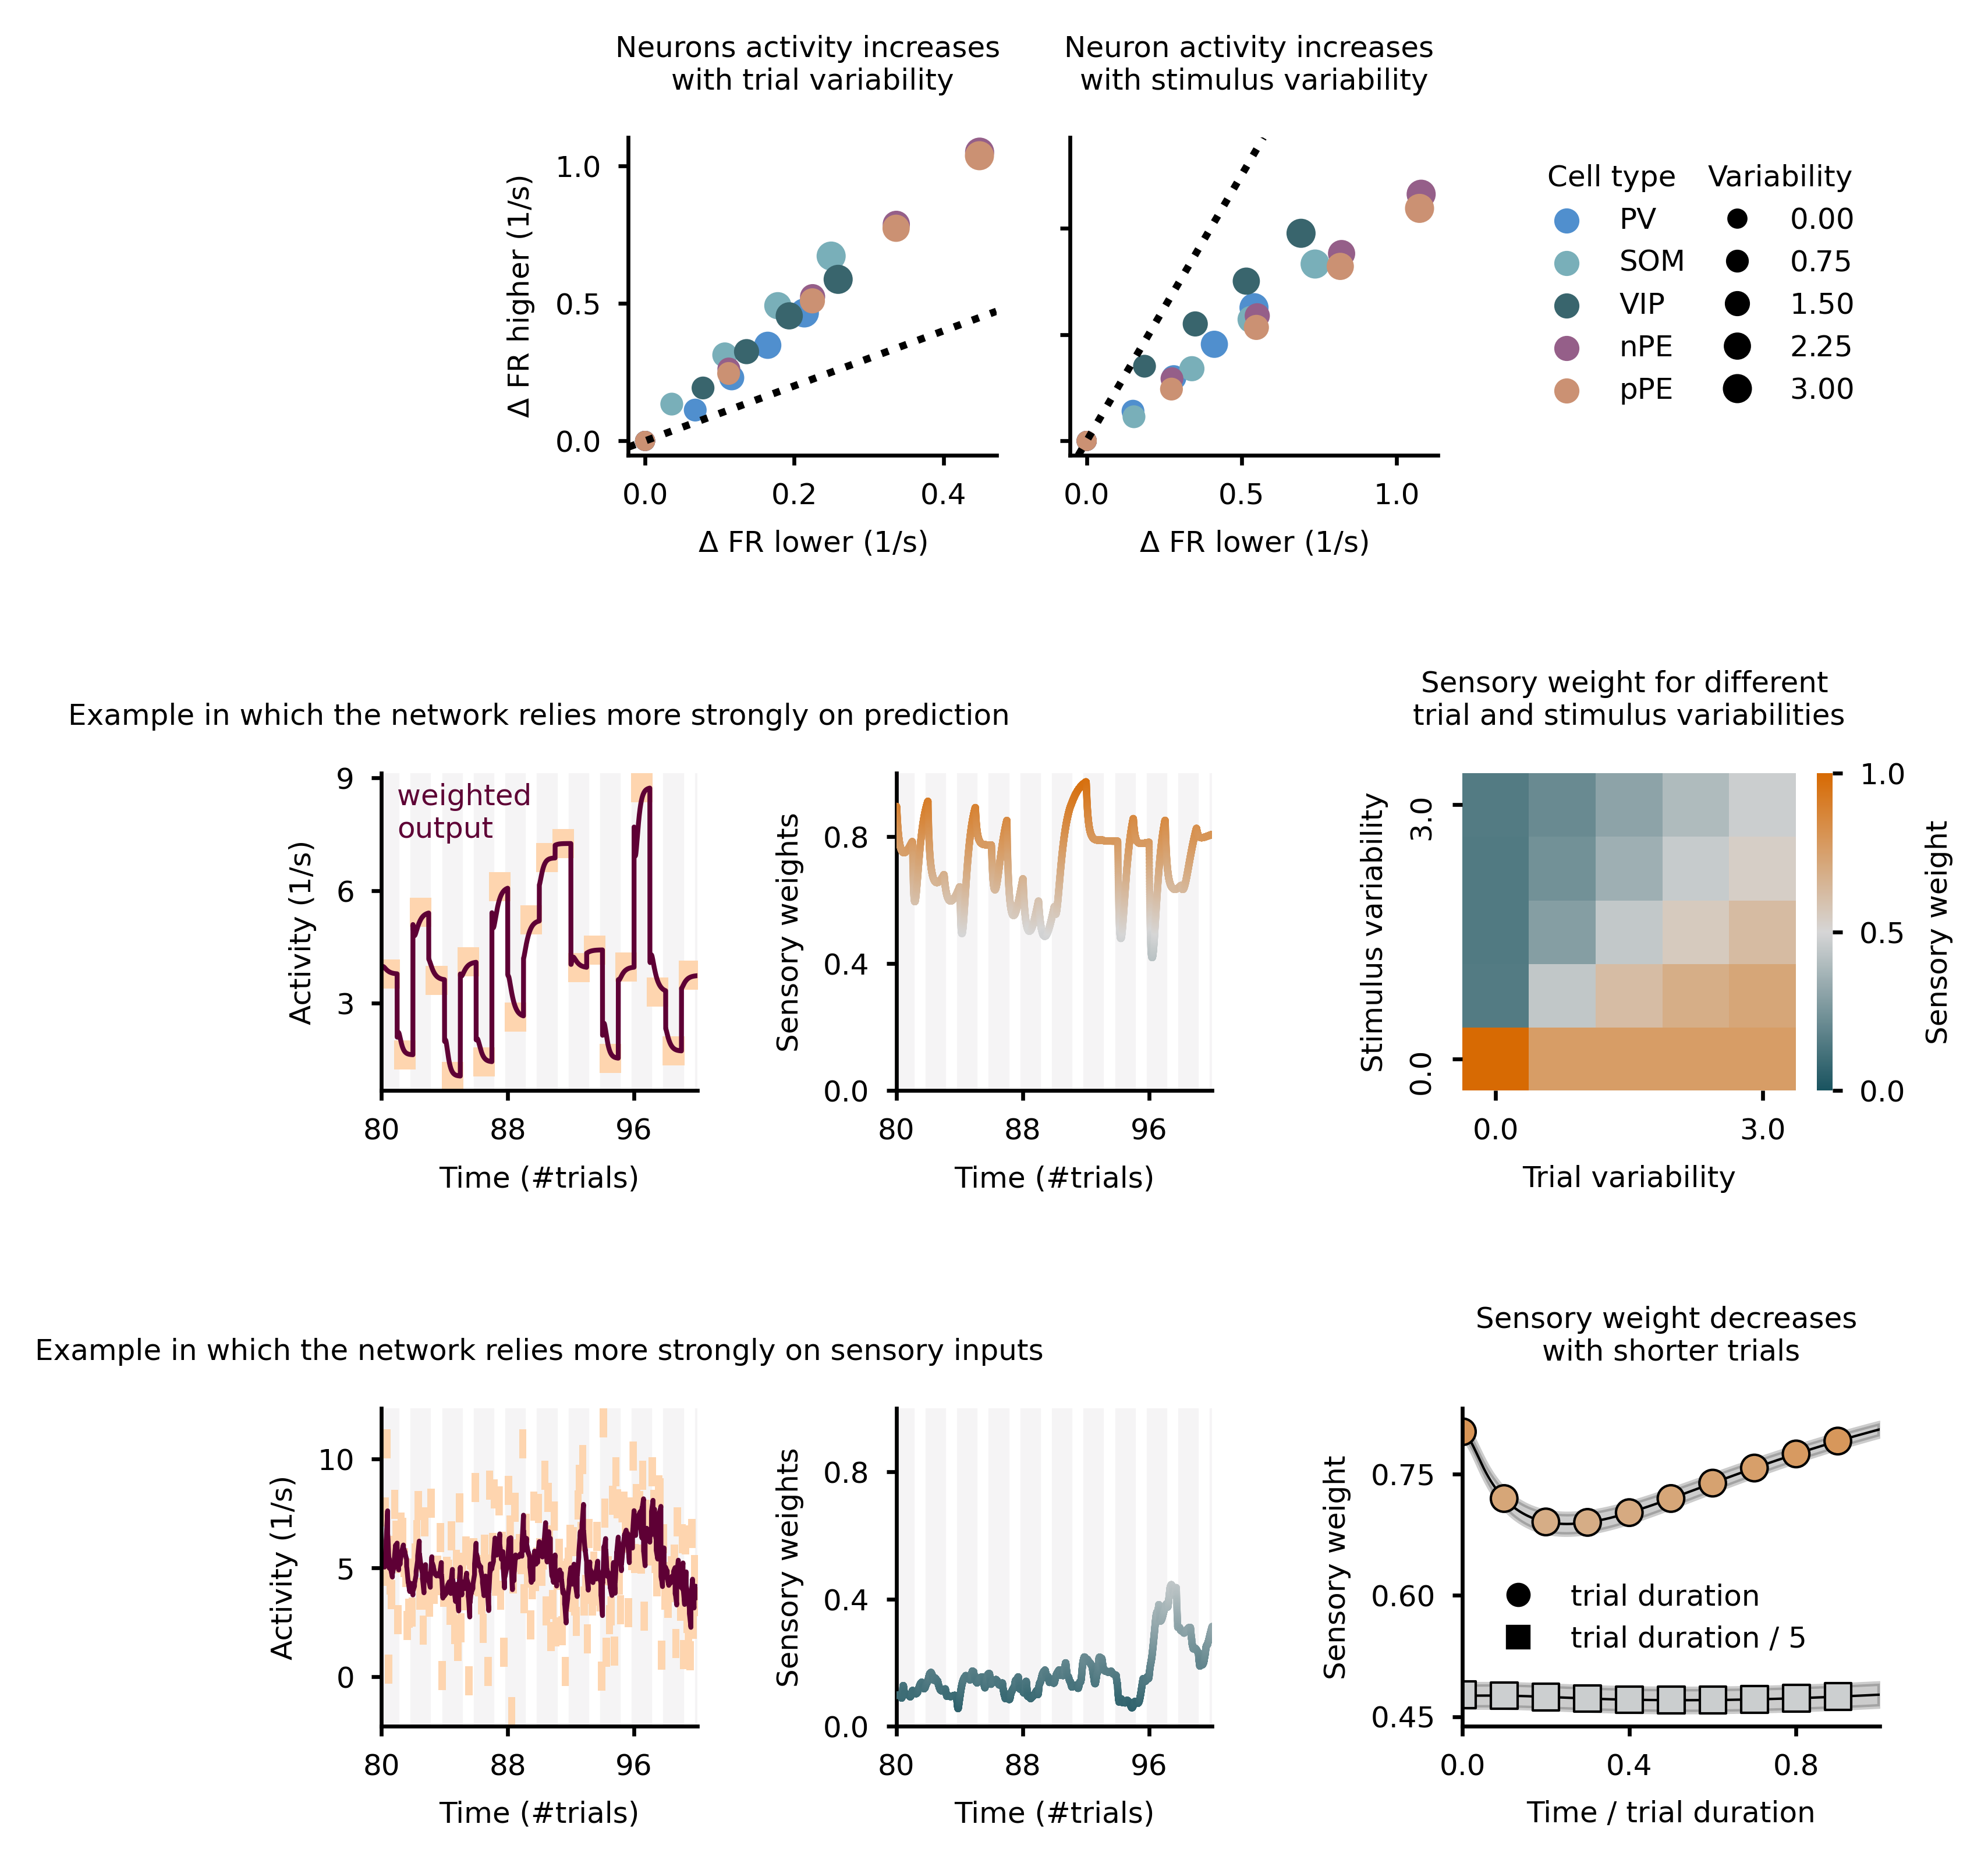
\includegraphics{../results/figures/final/Fig_3}}
    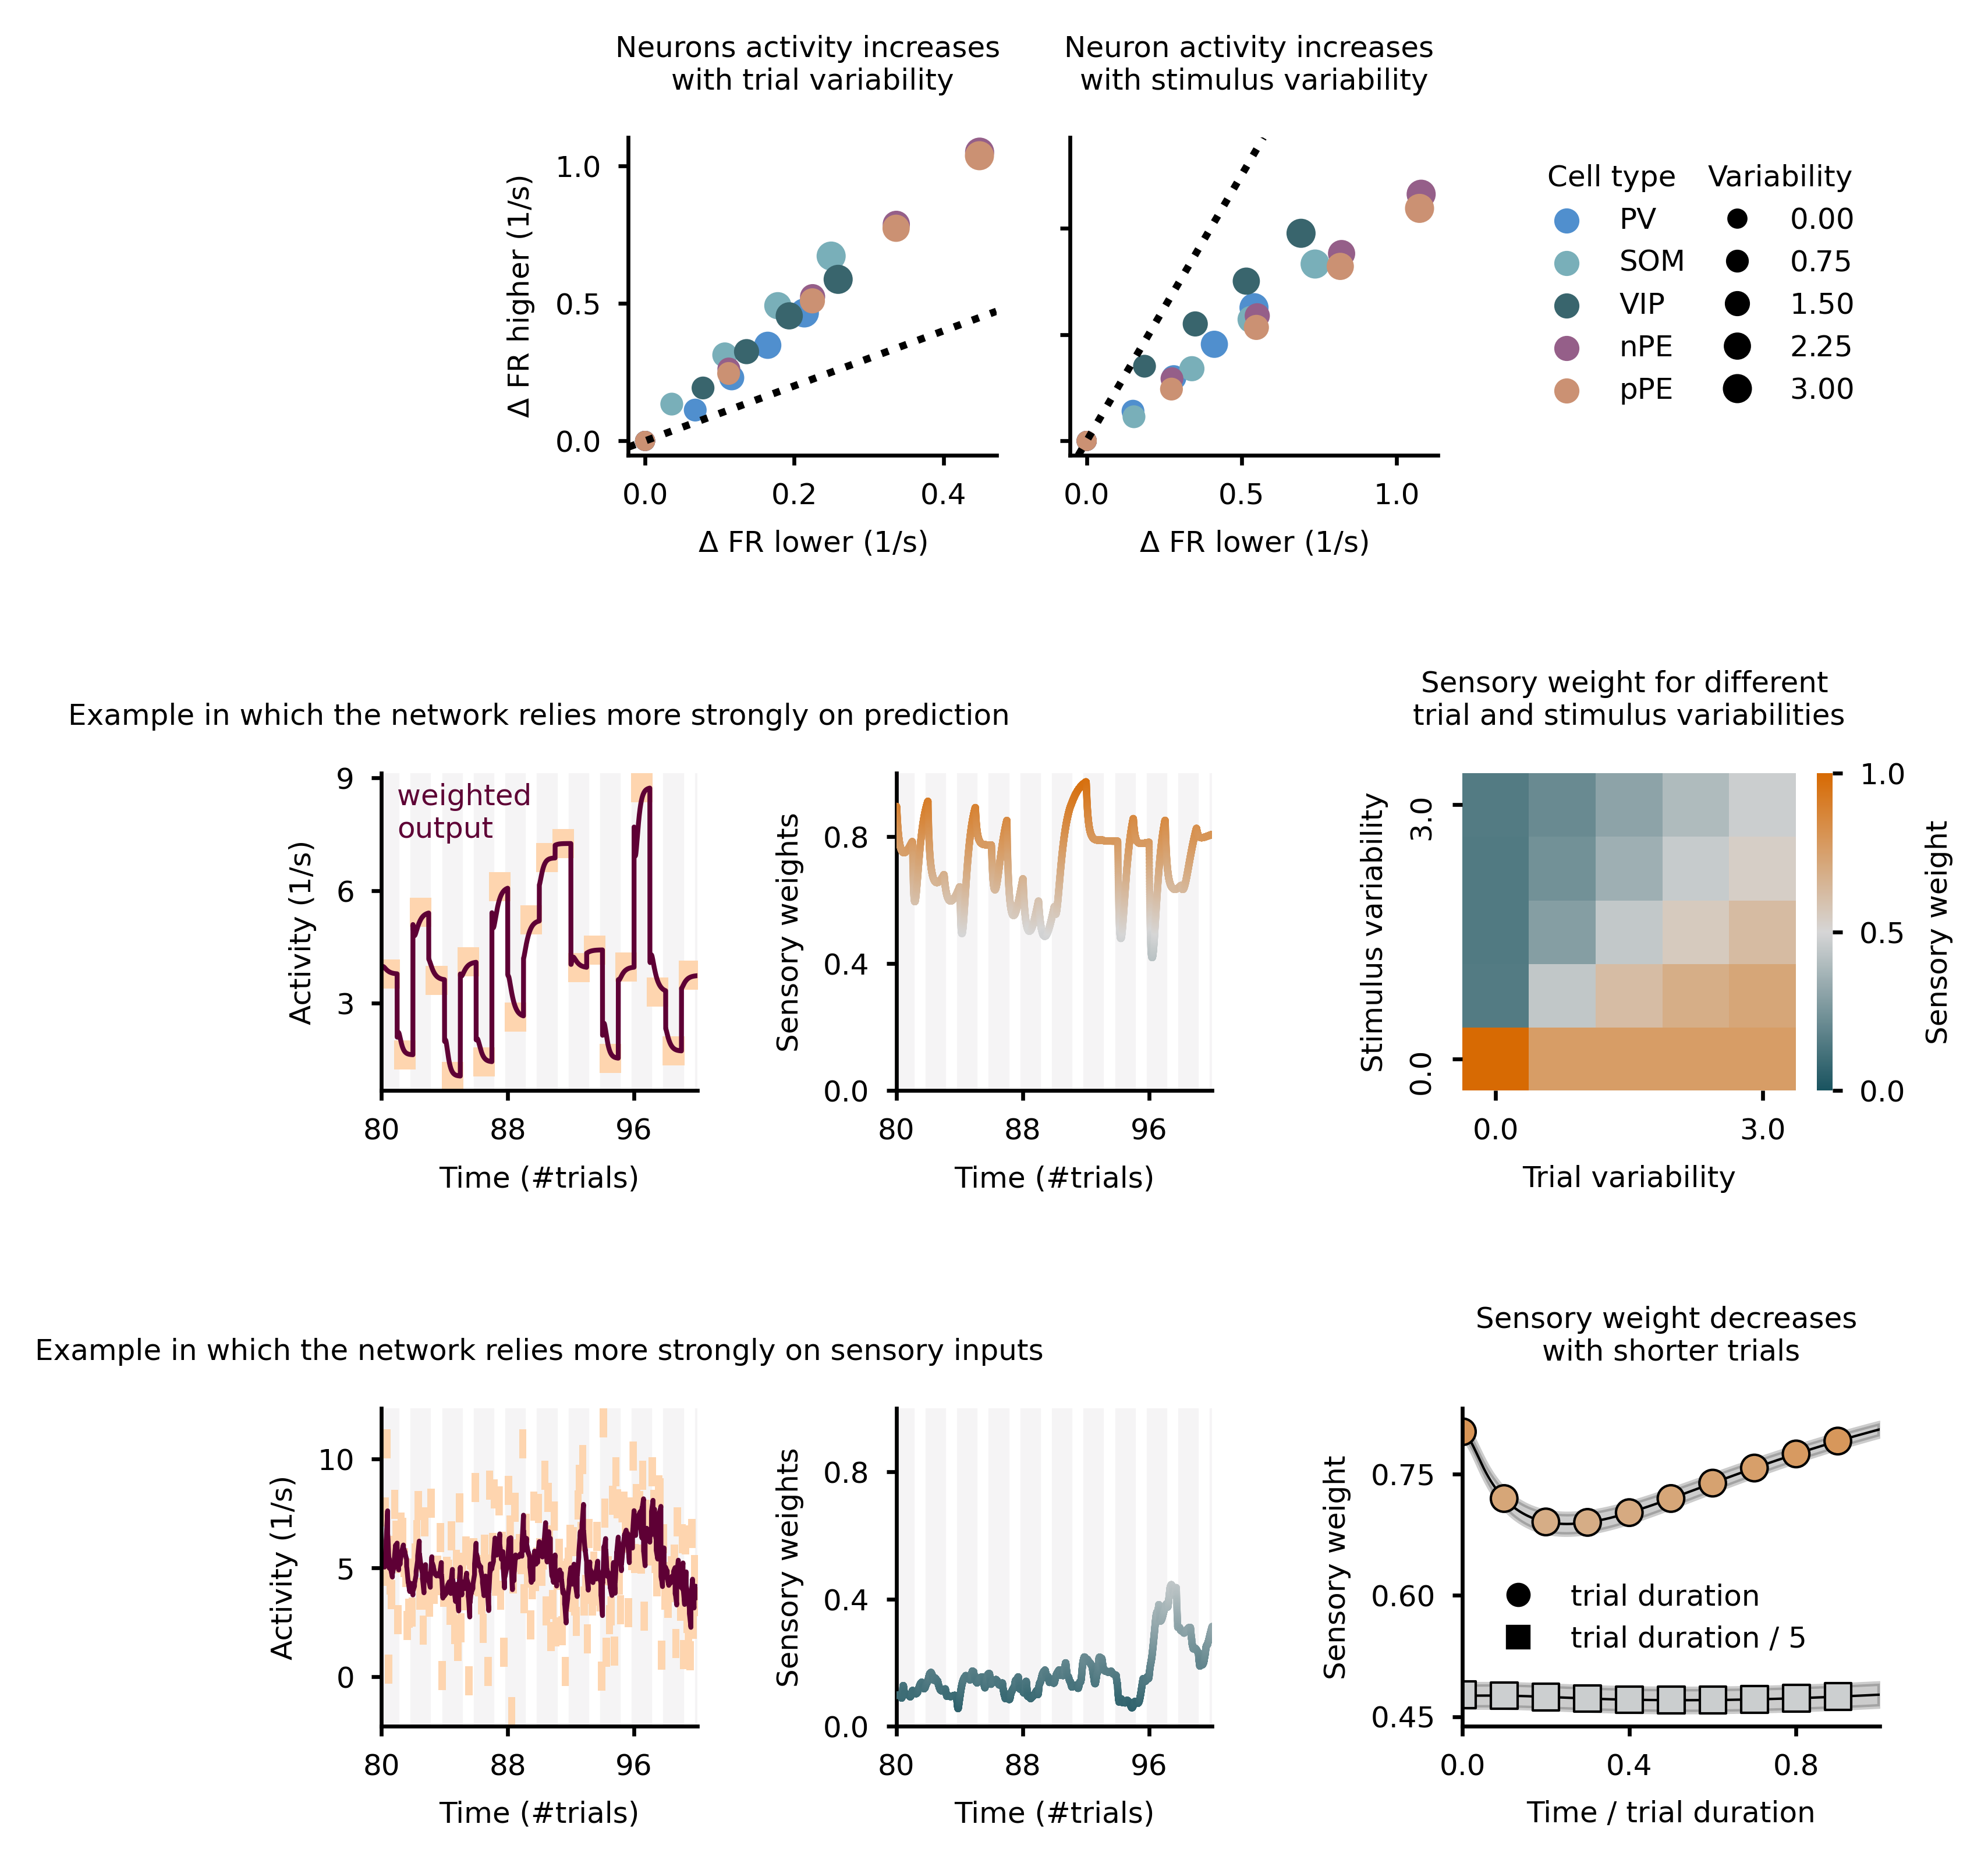
\includegraphics[width=1\linewidth]{../results/figures/final/Fig_3}
\caption{\footnotesize{\bf Estimating variances of sensory inputs and predictions with hierarchical PE circuits.\newline} 
{\bf (A)} Illustration of the stimulation protocol. Network is exposed to a sequence of stimuli (one stimulus per trial). To account for stimulus variability, each stimulus is represented by xxx stimulus values drawn from a normal distribution with mean $\mu_\mathrm{stim}$ and $\sigma_\mathrm{stim}^2$. To account for the volatility of the environment, in each trial the stimulus mean $\mu_\mathrm{stim}$ is drawn from a uniform distribution (denoted trial variability). Trial duration = xxx. 
{\bf (B)} Neuron activity increases with both stimulus and trial variability. Neurons in the lower PE circuit increase more strongly with stimulus variability. Neurons in the higher PE circuit increase more strongly with trial variability.
{\bf (C)} Limit case example in which the stimulus variability is low but the trial variability is high. Left: Illustration of the stimulation protocol. Middle: Weighted output follows closely the sensory stimuli. Right: Sensory weight (function of the variances, see text) close to 1, indicating that the network ignores the prediction. Input statistics: XXX.
{\bf (D)} Limit case example in which the stimulus variability is high but the trial variability is low. Left: Illustration of the stimulation protocol. Middle: Weighted output pushed towards the mean of the sensory stimuli. Right: Sensory weight close to zero, indicating that the network ignores the sensory stimuli. Input statistics: XXX.
{\bf (E)} Predictions are weighted more strongly when the stimulus variability is larger than the trial variability.
{\bf (F)} Predictions are weighted more strongly at the beginning of a new trial and quickly changing stimuli.
}
\label{fig:Fig_3}
\end{figure}
%

To test the network's ability to estimate the variances correctly, we stimulated the network with a sequence of inputs. In each trial one stimulus is shown to the network. To account for the stimulus variance, each stimulus is composed of \textit{n} constant values drawn from a normal distribution with mean $\mu_\mathrm{stim}$ and variance $\sigma_\mathrm{stim}^2$, and presented one after the other. To account for potential changes in the environment, in each trial, we draw $\mu_\mathrm{stim}$ from a uniform distribution (Fig. \ref{fig:Fig_3}A). Hence, the inputs change on two different time scales, with stimulus variability (faster time scale) and trial variability (slower time scale).

As expected, the neurons' activity increase for both stimulus and trial variances (Fig. \ref{fig:Fig_3}B). While the neurons in the lower PE circuit increase more strongly with stimulus variability, the neurons in the higher PE circuit increase more strongly with trial variability, indicating that the different subnetworks process different aspects of the inputs. We first consider two limit cases. In the first limit case, a different but low-variance stimulus is presented in each trial (Fig. \ref{fig:Fig_3}C, left). In line with the ideas of multisensory integration (XXX), the network should therefore follow the sensory inputs closely and ignore the predictions. When we arithmetically calculate the weighted output (Fig. \ref{fig:Fig_3}C, middle) based on the feedforward and feedback inputs, and the sensory weight (Fig. \ref{fig:Fig_3}C, right), the network correctly represents mostly the sensory input (for more details, see Methods). In the second limit case, the same but high-variance stimulus is presented in each trial (Fig. \ref{fig:Fig_3}D, left). According to the theory, the network should downscale the sensory feedforward input and weight the prediction more strongly. Indeed, the weighted output of the network shows a clear tendency to the mean of the stimuli (Fig. \ref{fig:Fig_3}D, middle), also reflected in the low sensory weight (Fig. \ref{fig:Fig_3}D, right). 

In a next step, to validate the network responses more broadly, we systematically varied the trial and stimulus variability independently. If both variances are similar, the sensory weight approaches \textit{0.5}, reflecting equal contribution of sensory inputs and predictions to the weighted output. Only if both variances are zero, the network represents the sensory input perfectly. In line with the limit case examples above, if the stimulus variance is larger than the trial variance, the network weights the prediction more strongly than the sensory input. This is reversed if the stimulus variance is smaller than the trial variance (Fig. \ref{fig:Fig_3}E). Because the network dynamically estimates the mean and variances of the sensory input and the prediction, the weighted output and the sensory weight changes accordingly when the input statistics changes (Fig. \ref{fig:Fig_3_S1}). 

The first limit case (Fig. \ref{fig:Fig_3}C) shows that even in a sensory-driven input regime, the prediction is weighted more at the beginning of a new trial than in the steady state. This is further confirmed in simulations in which the trail duration was shortened. For those simulations, the prediction even outweighs the sensory input, reflected in a very low sensory weight (Fig. \ref{fig:Fig_3}F). This suggests that predictions influence neural activity more significantly in experiments that rely on very fast stimulus changes. 

It has been shown [speculated?], that sensory inputs or predictions are overrated in some psychiatric disorders (XXX). We thus wondered which network properties might bias the estimation of the variances, and, consequently, the weighting of different input streams. In our network, the M neuron evolves faster in the lower subnetwork than in the higher one. We identified the speed at which the M neurons are updated with new information as a decisive factor in the integration of inputs. To show this, we varied the weights from the PE neurons onto the lower-level M neuron. If the M neuron evolves too slowly, the prediction is overrated. In contrast, if the M neuron incorporates new information too quickly, the sensory input is overrated (Fig. \ref{fig:Fig_3_S2}A). While the speeds at which the activity of the M neurons evolve may underlie pathological weighting of inputs, the precise activation function of the V neurons is less pivotal. When we replaced the squared activation function with a linear, rectified function, the V neurons do not encode the variance but the averaged absolute deviation of the sensory stimuli. However, the sensory weight is only slightly shifted to larger values for low trial/high stimulus variability (Fig. \ref{fig:Fig_3_S2}B). 

In summary, we show that the variances of both the sensory inputs and predictions thereof can be dynamically computed in networks comprising a lower and higher PE circuit. The model shows that predictions are trusted more strongly at the beginning of a new stimulus, and if sensory inputs are noisy on a short time scale while predictable on longer time scales.

% XXX Do we actually propose that predictions are sent up the hierarchy?

\subsection*{Biasing the weighting of sensory inputs and predictions by neuromodulators}
%
The brain's flexibility and adaptability are not least because a plethora of neuromodulators influence the activity of neurons in a variety of ways (XXX). A prominent target of neuromodulatory inputs is inhibitory neurons (Cardin 2019, XXX). Moreover, distinct interneuron types are differently (in-)activated by those neuromodulators. For instance, it has been shown that XXX (XXX). We, therefore, wondered if and how the weighting of sensory inputs and predictions thereof may be biased when neuromodulators activate distinct interneuron types.
%
\begin{figure}[t!]
	\centering
	\makebox[\textwidth][c]{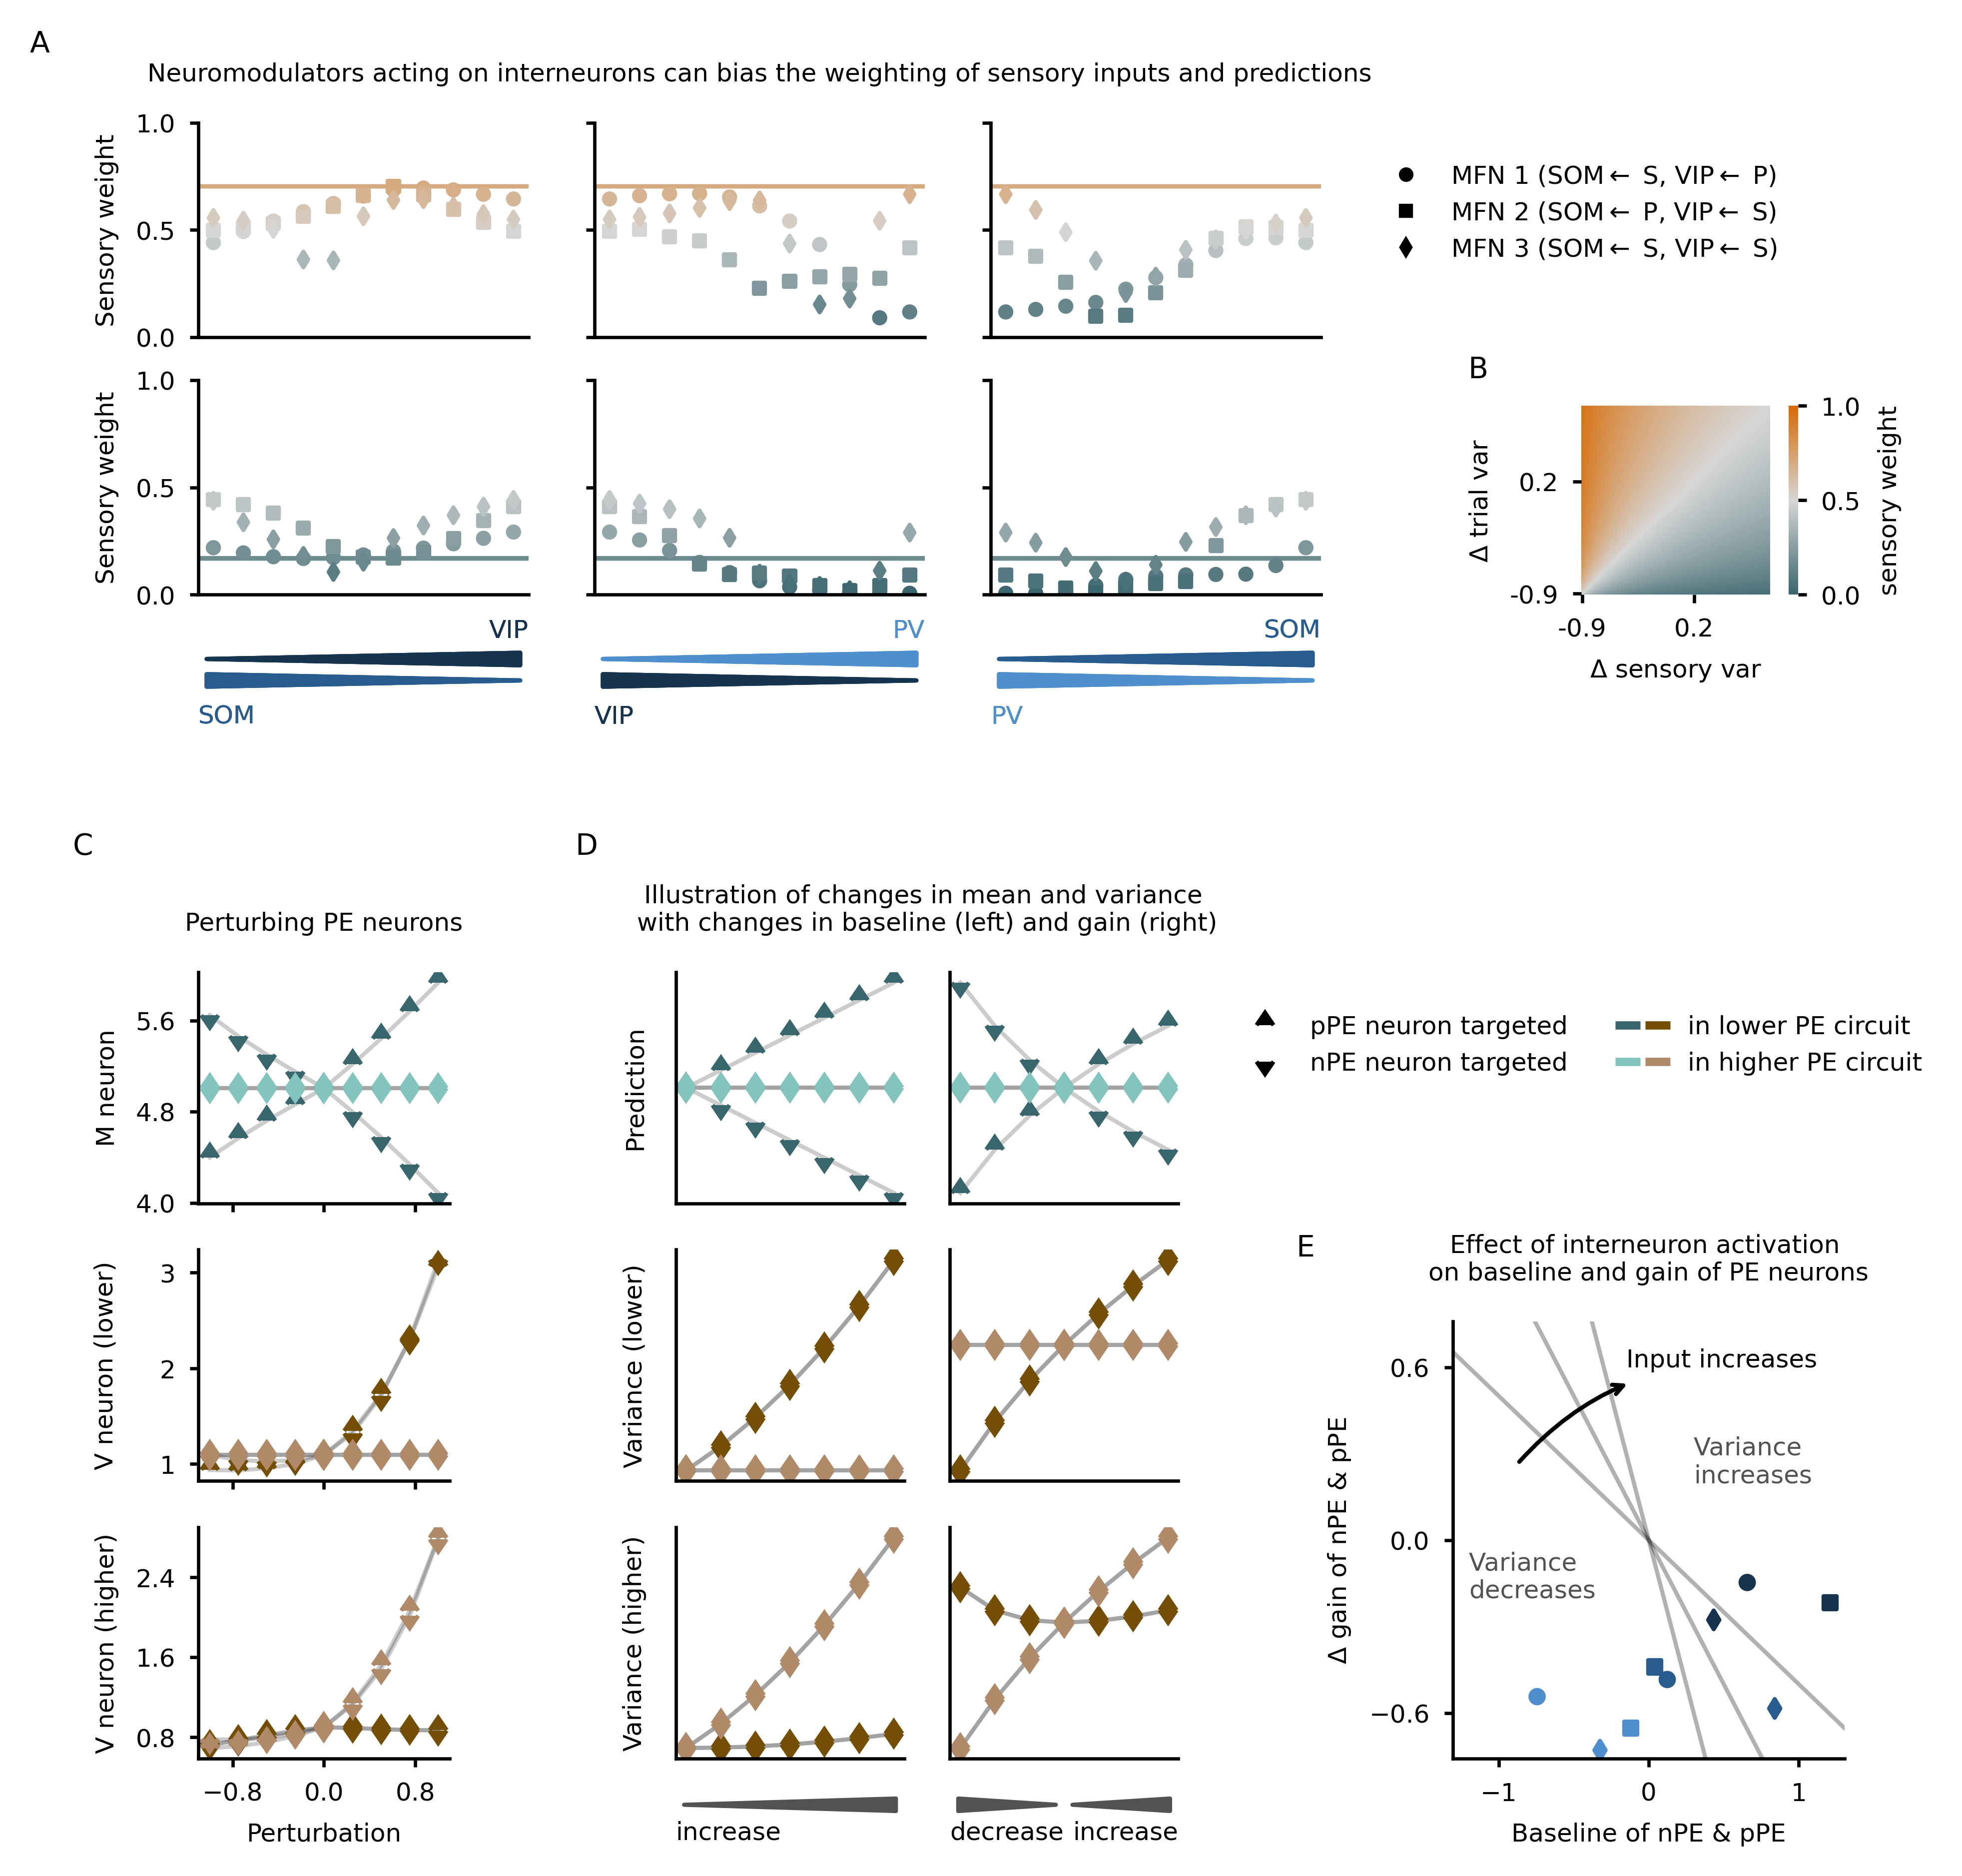
\includegraphics{../results/figures/final/Fig_4}}
    %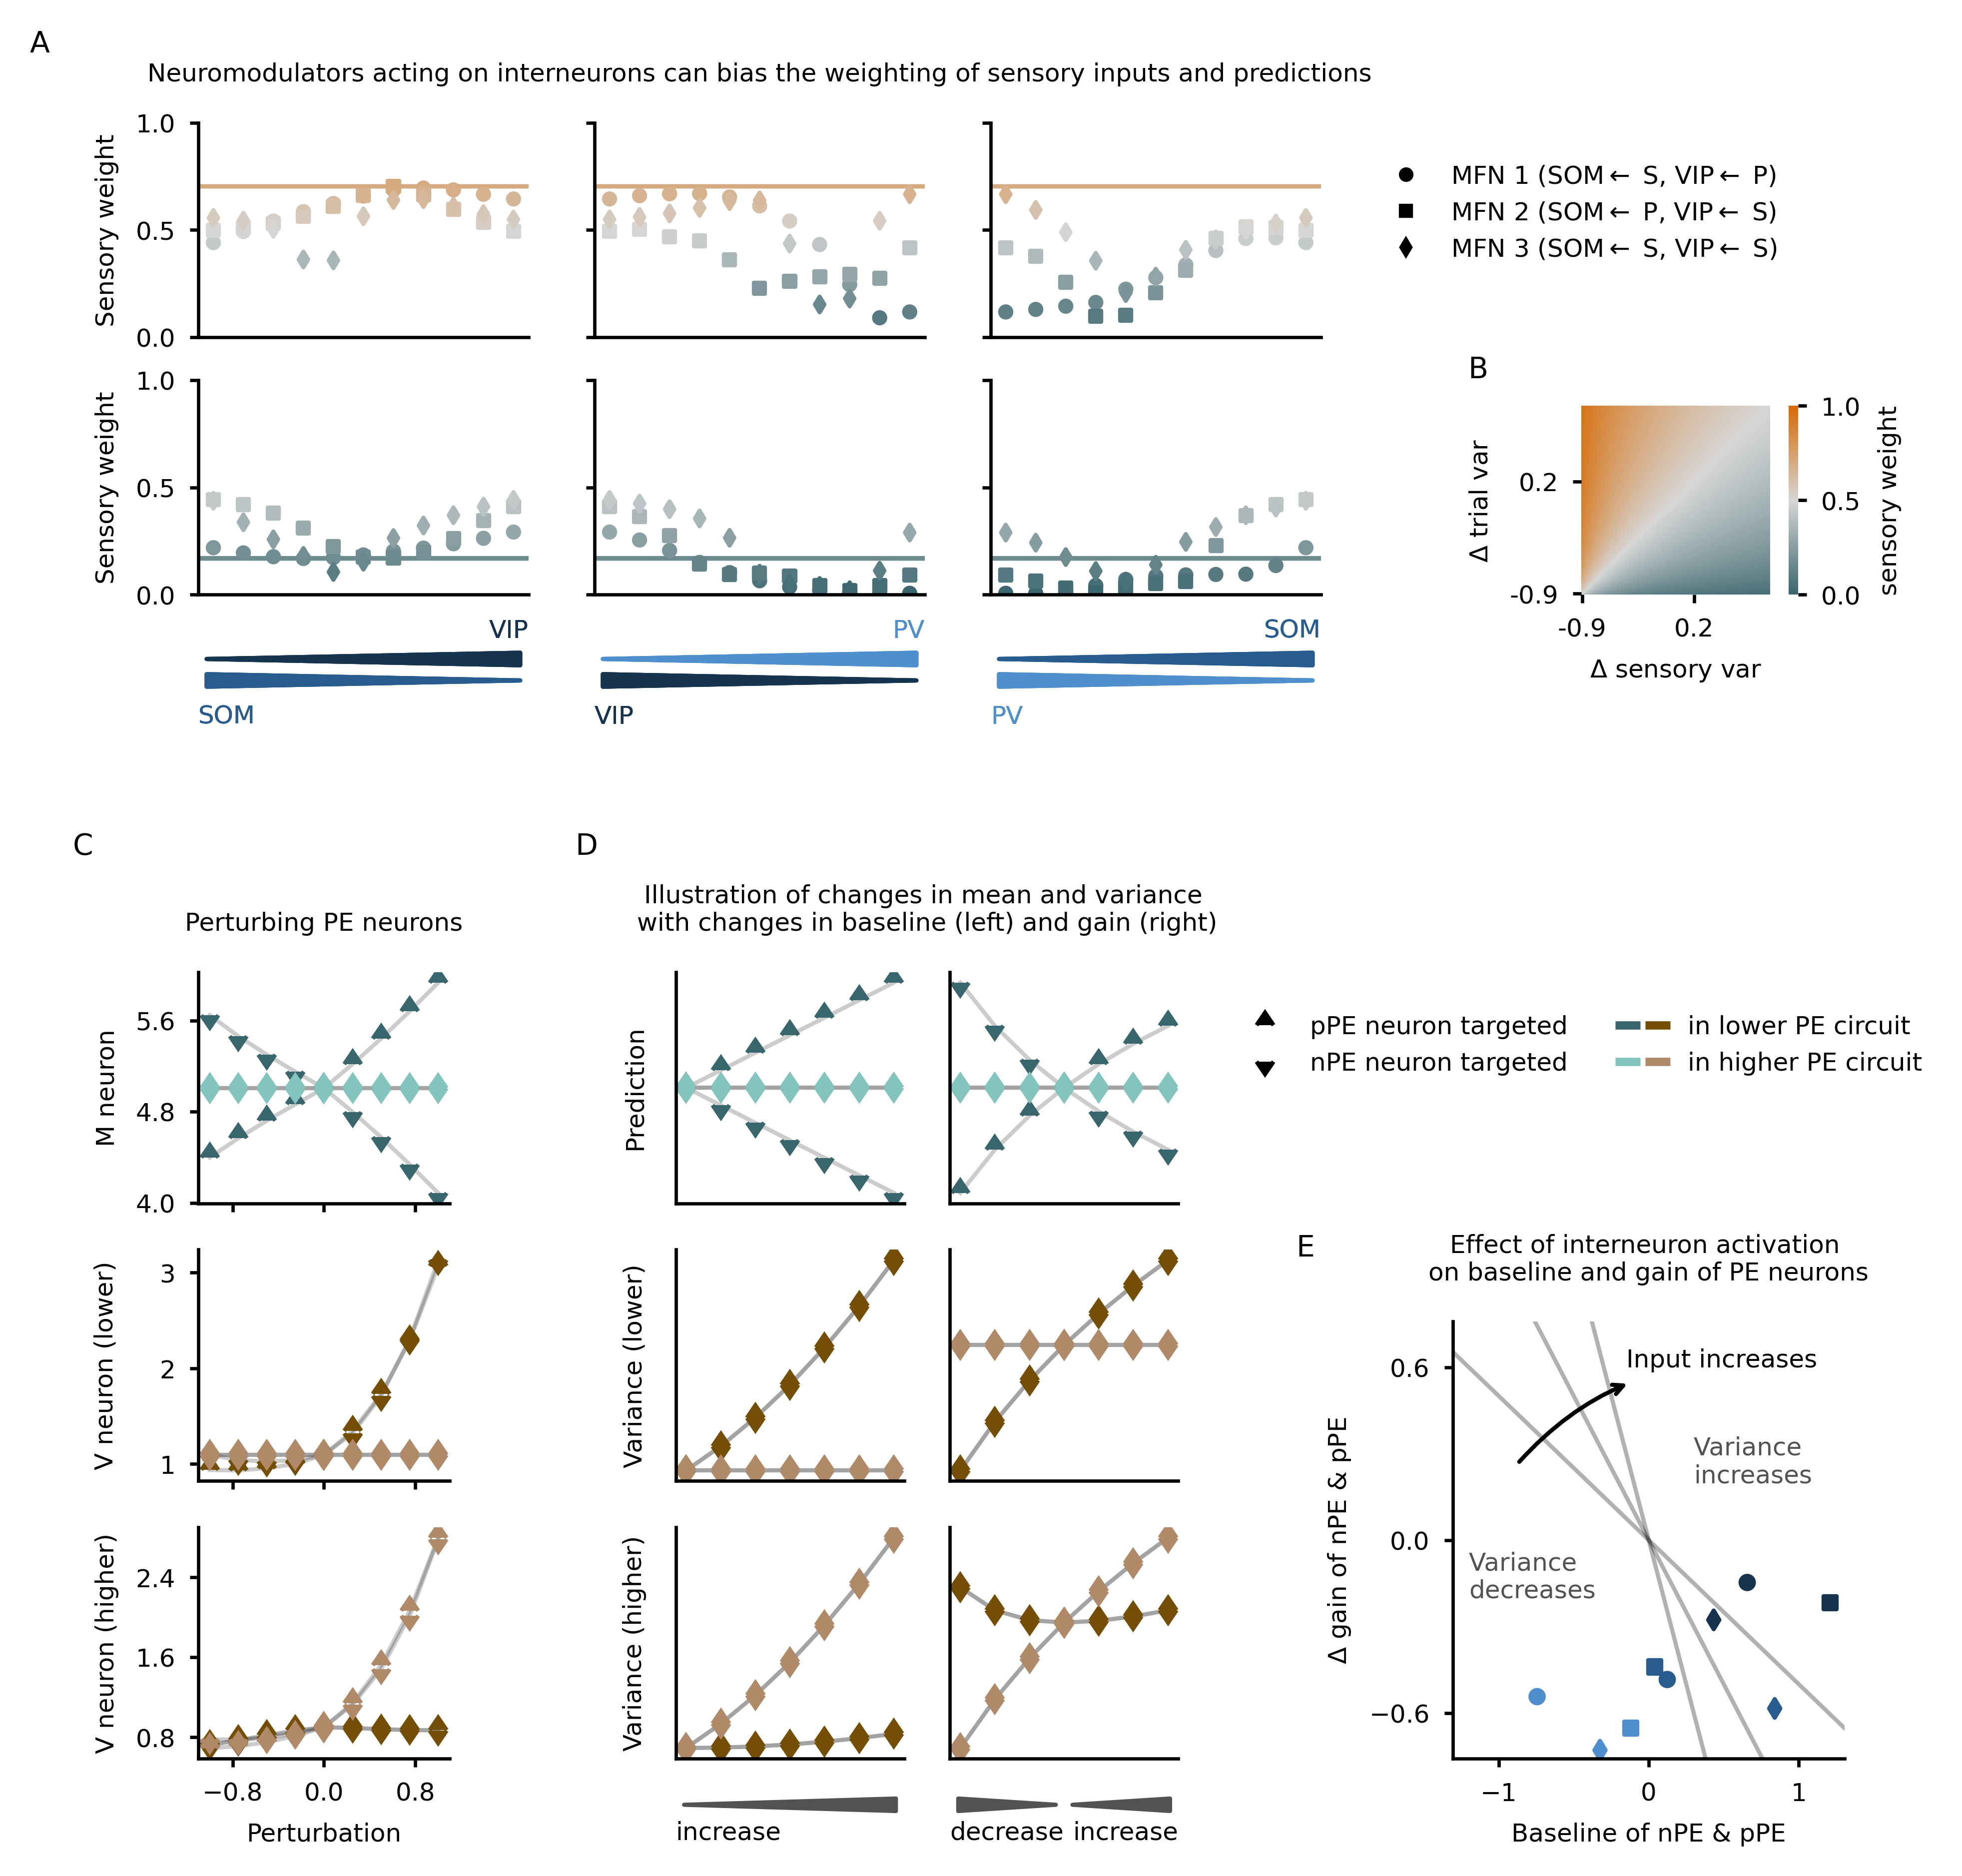
\includegraphics{../results/figures/final/Fig_4} % [width=1\linewidth]
\caption{\footnotesize{\bf Neuromodulator-based shifts in the weighting of sensory inputs and predictions.
\newline} 
{\bf (A)} Neuromodulators acting on the three interneurons may shift the weighting of sensory inputs and predictions. The changes depend on the type/s of interneurons targeted by the additional excitatory input emulating a neuromodulator (additional input = XXX). Considered are two limit cases (upper row: more sensory-driven before modulation, lower row: more prediction-driven before modulation). The combination of interneurons targeted is illustrated below. The results are shown for three different PE circuits, specified in the main text. 
{\bf (B)} Illustration showing how the sensory weight depends on changes in both the stimulus and trial variability.
{\bf (C)} The M and V neuron activities depend on the PE neuron activities. Hence, perturbing the nPE and pPE neurons must change the estimation of mean and variance. While stimulating the lower PE neurons affects both the lower and higher mean and variance estimation, stimulating the higher PE neurons only affects the V and M neurons in the same subnetwork.
{\bf (D)} Illustration of the mechanisms underlying the biased estimation of mean and variance when PE neurons are perturbed. Both changes in the baseline (left) and gain (right) of PE neurons can contribute to the changes observed in (C). Illustration based on toy model described in Methods.
{\bf (E)} Modulated interneurons change the weighting by changing the overall baseline and the overall gain of PE neurons (sum of changes in nPE and pPE neurons). Whether and how a neuromodulator changes the sensory weight, hence, depends on the interneuron targeted and the effect this interneuron has on baseline and gain of the PE neurons, which in turn does depend on the network it is embedded in.
}
\label{fig:Fig_4}
\end{figure}
%

To this end, we modeled the presence of neuromodulators by injecting an additional excitatory input into one or two interneuron types. We reasoned that the network effect of a neuromodulator not only depends on the interneuron type it targets but also on the inputs this neuron receives and the connections it makes with other neurons in the network. We, therefore, tested three different mean-field networks that differ with respect to the distribution of sensory inputs and predictions onto the interneurons, and the underlying connectivity. The commonality across those networks is that they exhibit an E/I balance of excitatory and inhibitory pathways onto the PE neurons (XXX). Across the different mean-field networks tested, activating a SOM or VIP neuron individually forces the networks to weigh both inputs more equally. As a consequence, predictions are overrated in a sensory-driven input regime. Similarly, sensory inputs are overrated in a prediction-driven input regime. Interestingly, when both interneuron types are activated to the same degree, this effect disappears (Fig. \ref{fig:Fig_4}A, left). In contrast, stimulating PV neurons biases the network's output towards predictions. This effect is even more pronounced when PV and SOM, or PV and VIP neurons are activated simultaneously (Fig. \ref{fig:Fig_4}A, middle and right). 

In the previous simulations, we assumed that a neuromodulator acts globally, that is, on the interneurons in both the lower and the higher PE circuit. While this agrees with experimental data showing that XXX (XXX), we note that neuromodulators may also act more locally. The effect of stimulating an interneuron type in the lower PE circuit on the sensory weight is mostly the opposite of activating the same interneuron in the higher PE circuit (Fig. \ref{fig:Fig_4_S1}). For instance, the sensory inputs are overrated when the higher-level VIP neuron is activated, while the prediction is overrated when the lower-level VIP neuron is activated. When VIP and SOM neurons are stimulated equally, the sensory weight remains unchanged, independently of which PE circuit is targeted by the neuromodulator. 

What are the mechanisms that give rise to these effects? And how do the combined local changes give rise to the global one observed in our network simulations? The sensory weight is chosen to be a function of the V neurons of the lower and higher PE circuit. Hence, any changes to the sensory weight result from changes to the neurons encoding the variances (Fig. \ref{fig:Fig_4}B). In our network, the V neurons only receive excitatory output synapses from PE neurons. Hence, any changes in the sensory weights upon activation of interneurons must be due to changes in the PE neurons. To disentangle the effect of nPE and pPE neurons, we perturbed those neurons individually in both the lower or higher subnetwork by injecting either an inhibitory or excitatory additional input (Fig. \ref{fig:Fig_4}C). Stimulating either PE neuron in the lower subnetwork increases the activity of the lower-level V neuron strongly. Moreover, the higher-level V neuron is also slightly affected. At first, this is counterintuitive because the V neuron in the higher subnetwork does not receive direct synapses from the PE neurons in the lower subnetwork. However, the activity of the lower-level M neuron encoding the prediction increases with an excitatory input onto the pPE neuron and decreases with an excitatory input onto the nPE neuron (the opposite is true for an inhibitory input). Because neurons in the higher PE circuit receive synapses from the lower-level M neuron, the activity of the higher-level V neuron is also affected. In contrast, stimulating either PE neuron in the higher subnetwork increases the activity of the higher-level V neuron but leaves the lower-level M and V neurons unaffected (Fig. \ref{fig:Fig_4}C).

Stimulating PE neurons may cause both an increase in the baseline activity and a change in the neuron's gain. To disentangle both effects, we illustrate each contribution separately using a mathematically tractable toy model (see Methods for more details). The variance estimated in the lower subnetwork increases with both increasing baseline and gain of the lower-level PE neurons. In contrast, when the gain of those PE neurons decreases, so does the variance. Similarly, the variance estimated in the higher subnetwork is equally influenced by changes in baseline and gain of the higher-level PE neurons. Moreover, changes to the baseline and the gain of the lower-level PE neurons increases the higher-level variance as a result of a biased prediction. Furthermore, the mean of the sensory stimuli is overpredicted (underpredicted) when the baseline or the gain of the lower-level pPE (nPE) neuron increases, or when the gain of the lower-level nPE (pPE) neuron decreases. In summary, if an interneuron causes an additional inhibitory input to a PE neuron, the neuron's gain is reduced. If an interneuron causes an additional disinhibitory input to a PE neuron, the neuron's baseline and gain are increased (Fig. \ref{fig:Fig_4}D).

This suggests that to understand the effect of neuromodulators on the sensory weight, we need to unravel the effect of interneuron activation on baseline and gain of PE neurons. To this end, we stimulated either PV, SOM, or VIP neurons independently for all three mean-field networks and measured the changes to baseline and gain of both PE neurons (Fig. \ref{fig:Fig_4}E). In all three networks tested, activating PV neurons decreases both quantities, leading to a decrease in the estimated variance (Fig. \ref{fig:Fig_4}E \& Fig. \ref{fig:Fig_4_S2}). Stimulating SOM or VIP neurons decreases the overall gain but increases the baseline activity of the PE neurons. Whether and how much the gain of the nPE or pPE neuron is reduced depends on the inputs onto SOM and VIP neurons, and the connectivity they make with other neurons in the network. Similarly, how much the baseline is elevated depends on the specifics of the mean-field network (Fig. \ref{fig:Fig_4}E \& Fig. \ref{fig:Fig_4_S2}). Hence, whether stimulating the SOM or VIP neuron decreases or increases the activity of the V neuron depends on the input statistics: for low-mean stimuli, the elevated baseline activity dominates the changes in the variance, while for high-mean stimuli the changes in the gain dominate. 

%XXX Summary ... effect of neuromodulators acting on INs on sensory weight best understood as combined effect on the baseline and gain of nPE and pPE neurons that in turn determine the activity of the V neuron. Those effects not ony depend on the target IN but also the network in which it is embedded, that is the connectivity and the inputs onto INs. Moreover, it depends on whether local or global. The effects of activation on lower is mainly the opposite of same in higher. However, the efefcts don't cancel each other in global modulation. Mostly because 1) V higher additionally changes due to changes in prediction but also 2) effects in higher are stronger !? and 3) 1/(1+(Vs + D)/(Vp + D)) ... that is it cannot cancel per se. Even though the underlying reasons for a change in the V neuron depends on the the network characteristics, there are some consistent changes in sensory weigt across MFN ... name

% in caption: you need to make sure that in e you used a perturbation of 1 and the mean and std of stimuli were ... the lines only illustrate that it depends on the input statistics. Of course, the markers would also change with other perturbaton strengths, would they though? Think through
% Mention that for V neuron (higher) the darker line is actually not horizontal (unaffected)!
% Mention that in BL illustration you need a factor to increase visibility ... (in caption)

\subsection*{The contraction bias as a result of the weighted integration of sensory inputs and predictions}
% 
The weighted integration of sensory inputs and predictions thereof manifests in all-day behavior, in the form of a phenomenon called \textit{contraction bias}. The contraction bias describes the tendency to overestimate sensory stimuli drawn from the lower end of a stimulus distribution and to underestimate stimuli drawn from the upper end of the same distribution (Fig. \ref{fig:Fig_5}A). This \textit{bias towards the mean} has been reported in different species and modalities (XXX). 
%
\begin{figure}[t!]
	\centering
    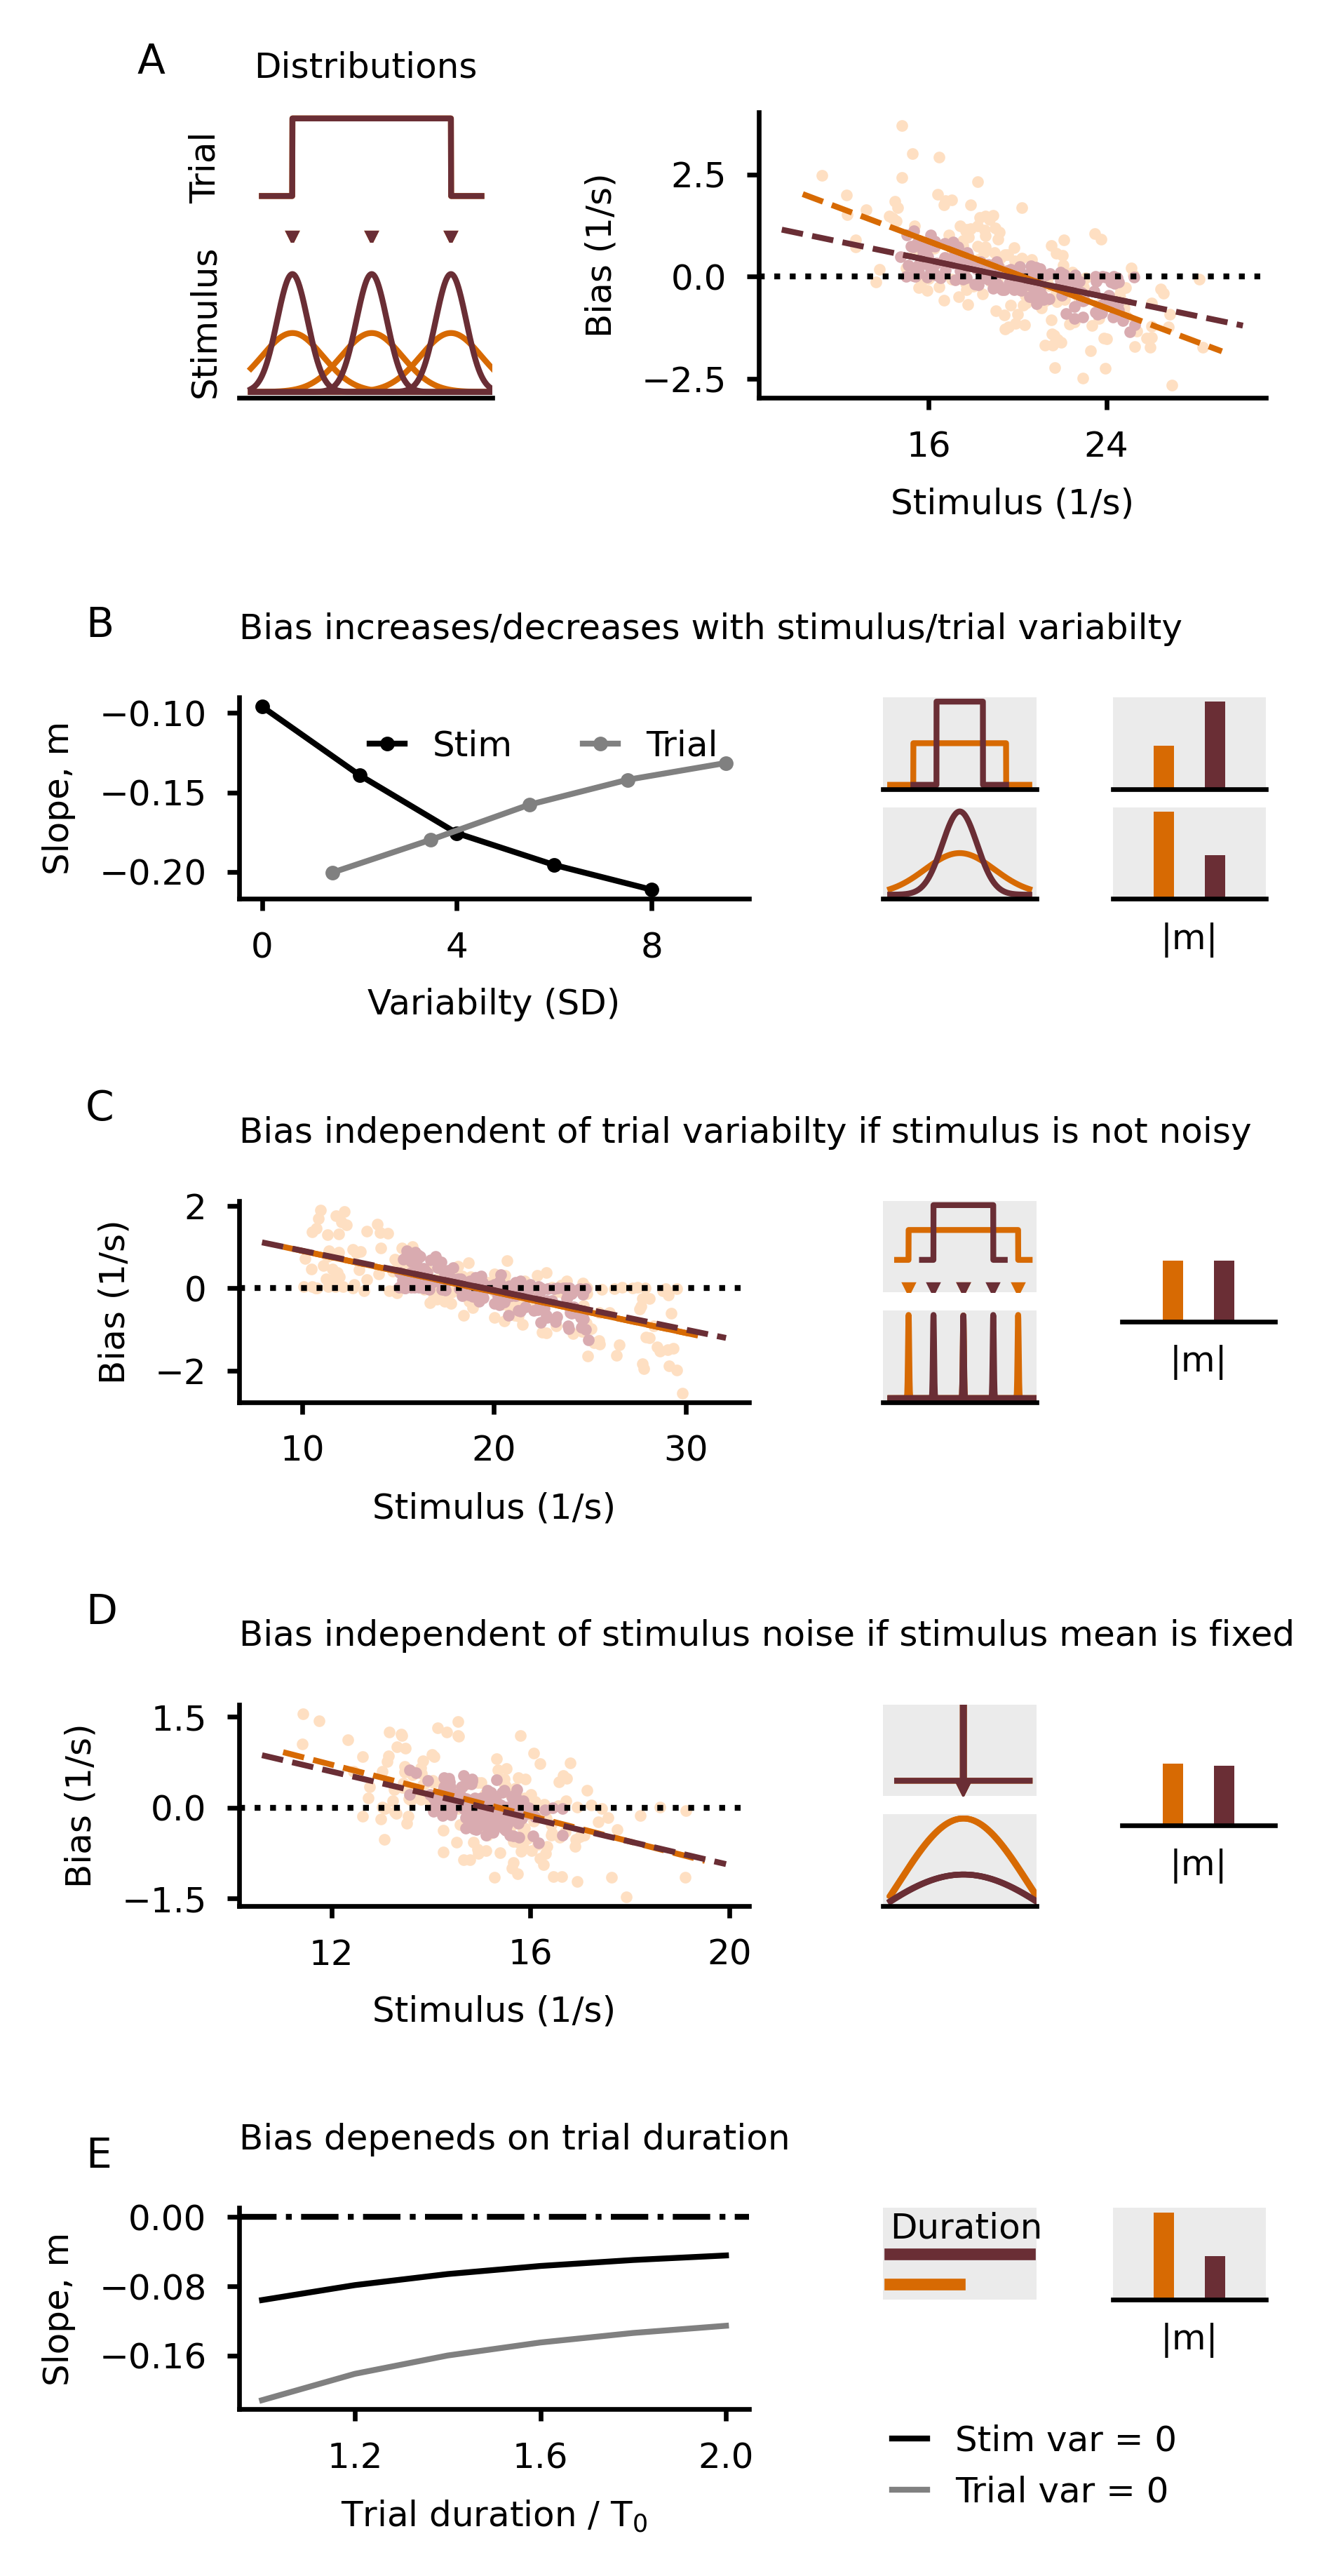
\includegraphics{../results/figures/final/Fig_5}
\caption{\footnotesize{\bf Mechanisms underlying the contraction bias.\newline} 
{\bf (A)} Illustration of the contraction bias. The estimated input is shifted towards the mean of the input distribution. Hence, a linear curve fitted to the data has a slope below 1 (left). The bias is biggest at the end of the stimulus distribution (right).
{\bf (B)} Contraction bias in the model. Left: Example for two different stimulus variabilities. Right: As a consequence of the sensory weight, the slope decreases with stimulus variability (bias increases) and increases with trial variability (bias decreases).  Stimulus statistics: XXX.
{\bf (C)} The bias is independent of trial variability when the stimulus variability is zero (left). Equally, the bias is independent of the stimulus variability when the trial variability is zero (right). Stimulus statistics: XXX.
{\bf (D)} The slope depends on the trial duration. If the sensory weight is 1, the slope is independent of the trail duration and the bias vanishes (dashed-dotted line). If the sensory weight is 0, the slope depends on the trial duration and only reaches 1 if the trial duration approaches infinity. 
{\bf (E)} To ensure a larger bias for stimuli drawn from the upper end of the stimulus distribution than from the lower end, scalar variability as observed experimentally is needed.
}
\label{fig:Fig_5}
\end{figure}
%

The weighted output of our network can be interpreted as a neural manifestation of the contraction bias (see Methods for a thorough analysis). The bias increases with stimulus variance (Fig. \ref{fig:Fig_5}B), decreasing the slope of the linear fit modeling the relationship between the true and estimated stimuli (Fig.\ref{fig:Fig_5}B, right; compare with Fig. \ref{fig:Fig_5}A). In contrast, the bias decreases with trial variance, so that the slope of the linear fit approaches 1 (Fig. \ref{fig:Fig_5}B right).

What are the underlying network factors that contribute to this phenomenon? To disentangle the potentially different sources of the bias, we first simulated a network without stimulus variability (variance set to zero) for two different trial variabilities. In this case, a contraction bias emerges but is independent of the volatility of the environment (Fig. \ref{fig:Fig_5}C, left). We show mathematically that the bias results from the transient neuron activity before reaching a steady state, and vanishes if the trial duration approaches infinity (see Methods for more details, and Fig. \ref{fig:Fig_5}D). We next resume the limit case in which the same but high-variance stimulus is shown in every trial. In this case, the weighted output exhibits a contraction bias that is largely independent of the stimulus variance (Fig. \ref{fig:Fig_5}C, right and Fig. \ref{fig:Fig_5}D). As shown mathematically (see Methods), the bias results from the finite trial duration and the tendency to weight the prediction more strongly than the sensory inputs. 
% Maybe show the limit for both cases and show the theoretical values for each T as well ... ?

So far, we assumed that the stimulus variance is independent of the trial mean. A consequence of this choice is that the bias on either end of the stimulus distribution is largely the same (but with reversed signs). However, behavioral (neural?) data (XXX) shows that the bias increases for stimuli drawn from the upper end of the distribution, a phenomenon usually attributed to \textit{scalar variability}. To capture this in the model, we assume that the stimulus standard deviation linearly increases with the trial mean. In these simulations, as expected, the bias increases for a stimulus distribution shifted to higher trial means (Fig. \ref{fig:Fig_5}E).

In summary, the weighted integration of sensory inputs and predictions can be interpreted as a neural manifestation of the contraction bias. Both stimulus and trial variability contribute to the contraction bias but the underlying mechanisms differ. 

% Enough? This section seems rather short! Should we do more, like making predictions about what would happen with the bias if neuromodulators activate INs? Like going back?


\section*{Discussion}

We solved the brain.

% At the end, or in between talk about changes in PE neurons directly that you have currently in Fig. 3 SX ... I copy the part of the last paragraph here as inspiration :
% For some psychiatric disorders, it has been shown that the weighting of sensory inputs and predictions thereof is impaired (XXX), leading to an overweighting of one of these signals. Moreover, it has been hypothesised that factors like stress or cognitive load may also influence the processing of feedforward and feedback inputs (XXX). ... Another factor that may contribute to a distorted weighting is the baseline activity of PE neurons that was set to zero in our model, in line with very low spontaneous firing rates of excitatory neurons in rodent primary sensory areas (XXX). Increasing this baseline activity for the nPE neuron (Fig. SXXX), pPE neuron (Fig. SXXX) or both pushes the network to weight sensory stimuli and predictions more equally. We speculate that an increase of baseline activity may be a natural result of an increased cognitive load or stress. 

% mention Pakan paper

\section*{Models and methods}
%
\subsection*{Network model}
The mean-field network model consists of a \textit{lower} and \textit{higher} PE circuit (Fig. \ref{fig:Fig_1}). Each PE circuit contains an excitatory nPE neuron and pPE neuron ($\mathrm{N}_\mathrm{nPE} = \mathrm{N}_\mathrm{pPE} = 1$), as well as inhibitory neurons. The inhibitory neurons comprise PV, SOM and VIP neurons ($\mathrm{N}_\mathrm{SOM} = \mathrm{N}_\mathrm{VIP} = 1$, $\mathrm{N}_\mathrm{PV} = 2$). In addition to the core PE circuit, each subnetwork also includes one memory neuron $M$ and one variance neuron $V$. 

The excitatory neurons in the PE circuit are simulated as two coupled point compartments, representing the soma and the dendrites of elongated pyramidal cells. All other neurons are modeled as point neurons. The activities of all neurons are represented by a set of differential equations describing the network dynamics. 

The dynamics of the neurons in the lower and higher PE circuits ($\underline{r}_\mathrm{PE}^\mathrm{low}$ and $\underline{r}_\mathrm{PE}^\mathrm{high}$) are given by
%
\begin{align}
\underline{r}_\mathrm{PE}^\mathrm{low} = & \left[ \underline{h}_\mathrm{PE}^\mathrm{low} \right]_+ \nonumber\\
%
\underline{r}_\mathrm{PE}^\mathrm{high} = & \left[ \underline{h}_\mathrm{PE}^\mathrm{high} \right]_+ 
\end{align}
%
with
%
\begin{align}
T \cdot \underline{\dot{h}}_\mathrm{PE}^\mathrm{low} =& -\underline{h}_\mathrm{PE}^\mathrm{low} + W_\mathrm{PE\leftarrow PE} \cdot \underline{r}_\mathrm{PE}^\mathrm{low} + \underline{w}_\mathrm{PE\leftarrow M} \cdot r_\mathrm{M}^\mathrm{low} + \underline{w}_\mathrm{PE\leftarrow FF} \cdot s + \underline{I}_\mathrm{PE} \nonumber\\
%
T \cdot \underline{\dot{h}}_\mathrm{PE}^\mathrm{high} =& -\underline{h}_\mathrm{PE}^\mathrm{high} + W_\mathrm{PE\leftarrow PE} \cdot \underline{r}_\mathrm{PE}^\mathrm{high} + \underline{w}_\mathrm{PE\leftarrow M} \cdot r_\mathrm{M}^\mathrm{high} + \underline{w}_\mathrm{PE\leftarrow FF} \cdot r_\mathrm{M}^\mathrm{low} + \underline{I}_\mathrm{PE}.
%
\end{align}
%
We follow the notation that column and row vectors are indicated by small letters with an underscore $\underline{\bullet}$, matrices are denoted by capital letters, and scalars are given by small letters without an underscore. Furthermore, a time derivative (e.g., $\frac{dx}{dt}$) is denoted by a dot above the letter (e.g., $\dot{x}$). The rate vector $\underline{r}_\mathrm{PE}^\mathrm{loc} = \left[r_\mathrm{nE}^\mathrm{loc},\ r_\mathrm{pE}^\mathrm{loc},\ r_\mathrm{nD}^\mathrm{loc},\ r_\mathrm{pD}^\mathrm{loc},\ r_\mathrm{PV_1}^\mathrm{loc}, r_\mathrm{PV_2}^\mathrm{loc},\ r_\mathrm{SOM}^\mathrm{loc}, r_\mathrm{VIP}^\mathrm{loc} \right]$  with $\mathrm{loc} \in [\mathrm{low}, \mathrm{high}]$ contains the activities of all neurons or compartments in the PE circuit (soma of nPE/pPE neurons: nE/pE, dendrites of nPE/pPE neurons: nD/pD). The network receives time-dependent stimuli $s$ and neuron/compartment-specific external background input $\underline{I}_\mathrm{PE}$. The connection strengths between the \textit{pre}-synaptic neuron (population) and the neurons of the PE circuit are denoted by $W_\mathrm{PE\leftarrow pre}$ and $\underline{w}_{\mathrm{PE} \leftarrow pre}$, respectively. The activities of the neurons evolve with time constants contained in $T$.

The activities of the lower and higher M neuron evolve according to a perfect integrator. The memory neurons receive synapses from both nPE and pPE neurons of the same subnetwork,
%
\begin{align}
\dot{r}_\mathrm{M}^\mathrm{low} =& \underline{w}_\mathrm{M \leftarrow PE}^\mathrm{low} \cdot \underline{r}_\mathrm{PE}^\mathrm{low} = w_\mathrm{M \leftarrow pPE}^\mathrm{low} \cdot r_\mathrm{pPE}^\mathrm{low} - w_\mathrm{M \leftarrow nPE}^\mathrm{low} \cdot r_\mathrm{nPE}^\mathrm{low} \nonumber \\
%
\dot{r}_\mathrm{M}^\mathrm{high} =& \underline{w}_\mathrm{M \leftarrow PE} ^\mathrm{high} \cdot \underline{r}_\mathrm{PE}^\mathrm{high} = w_\mathrm{M \leftarrow pPE}^\mathrm{high}  \cdot r_\mathrm{pPE}^\mathrm{high} - w_\mathrm{M \leftarrow nPE}^\mathrm{high}  \cdot r_\mathrm{nPE}^\mathrm{high} .
\end{align}
%

The activities of the lower and higher V neuron evolve according to a leaky integrator with quadratic activation function. The variance neurons receive synapses from both nPE and pPE neurons of the same subnetwork,
%
\begin{align}
\tau_\mathrm{V}^\mathrm{low} \cdot \dot{r}_\mathrm{V}^\mathrm{low} =& - r_\mathrm{V}^\mathrm{low} + \left( \underline{w}_\mathrm{V \leftarrow PE} \cdot \underline{r}_\mathrm{PE}^\mathrm{low}\right)^2 = - r_\mathrm{V}^\mathrm{low} + \left( w_\mathrm{V \leftarrow pPE} \cdot r_\mathrm{pPE}^\mathrm{low}\ + w_\mathrm{V \leftarrow nPE} \cdot r_\mathrm{nPE}^\mathrm{low}\right)^2 \nonumber\\
%
\tau_\mathrm{V}^\mathrm{high} \cdot \dot{r}_\mathrm{V}^\mathrm{high} =& - r_\mathrm{V}^\mathrm{high} + \left( \underline{w}_\mathrm{V \leftarrow PE} \cdot \underline{r}_\mathrm{PE}^\mathrm{high}\right)^2 = - r_\mathrm{V}^\mathrm{high} + \left( w_\mathrm{V \leftarrow pPE} \cdot r_\mathrm{pPE}^\mathrm{high}\ + w_\mathrm{V \leftarrow nPE} \cdot r_\mathrm{nPE}^\mathrm{high}\right)^2.
\end{align} 
%
All values for neuron and network parameters, details on the model equations, as well as supporting analyses can be found in SI XXX.

\subsection*{Weighting of sensory inputs and predictions}
%
We arithmetically calculate the weighted output of sensory inputs and predictions, $r_\mathrm{out}$, based on Bayesian multisensory integration (XXX),
%
\begin{align}
r_\mathrm{out} = \alpha \cdot s + (1-\alpha) \cdot r_\mathrm{M}^\mathrm{low},
\end{align}
%
where $\alpha$ denotes the reliability of the sensory input and is given by 
%
\begin{align}
\alpha &= \left( 1 + \frac{r_\mathrm{V}^\mathrm{low}}{r_\mathrm{V}^\mathrm{high}} \right)^{-1}.
\end{align}


\subsection*{Inputs}
%
The network receives feedforward stimuli of duration XXX that can change from trial to trial (one stimulus per trial). To account for noise, each stimulus is composed of N$_\mathrm{val}$ piece-wise constant values drawn from a normal distribution with mean XXX and standard deviation XXX. To account for changes in the environment, the mean of the normal distribution is drawn from a uniform distribution with mean XXX and standard deviation XXX. The parameterisation of both distributions varies across the experiments. All stimulus/input parameters can be found in SI XXX.

\subsection*{Simulations}
%
All simulations were performed in customized Python code written by LH. Differential equations were numerically integrated using a 2\textsuperscript{nd}-order Runge-Kutta method with time steps ranging between $xx$ and $xxx$ ms. All neurons were initialized with $r=0/s$. We defined the steady-state firing rate per stimulus as the activity in the last XXXX ms of stimulus presentation. Further details and values for simulation parameters can be found in SI XXX.


\section*{Acknowledgments}
%
%We are grateful to Vezha Boboeva, Douglas Feitosa Tom\'e, J\'ulia Gallinaro and Klara Kaleb for helpful comments on earlier versions of this manuscript, and we want to thank all members of the Clopath lab for discussion and support. This work was supported by BBSRC BB/N013956/1, BB/N019008/1, Wellcome Trust 200790/Z/16/Z, Simons Foundation 564408 and EPSRC EP/R035806/1.

\bibliographystyle{naturemag} %{plainnat}
\bibliography{../References_Mismatch}



%%%%%%%%%%%%%%%%%%%%%%%%%%%%%%%%%%%%%%%%%%%%%%%%%%%%%%%%%%%%
%%% APPENDICES
%%%%%%%%%%%%%%%%%%%%%%%%%%%%%%%%%%%%%%%%%%%%%%%%%%%%%%%%%%%%


\clearpage
\appendix


\tableofcontents
\section{Detailed Methods}

XXX

\subsection{Network model}
%
The network model consists of a \textit{lower} and \textit{higher} mean-field PE circuit (Fig. \ref{fig:Fig_1}). Each PE circuit contains an excitatory nPE neuron and pPE neuron ($\mathrm{N}_\mathrm{nPE} = \mathrm{N}_\mathrm{pPE} = 1$), as well as inhibitory neurons. The inhibitory neurons comprise PV, SOM and VIP neurons ($\mathrm{N}_\mathrm{SOM} = \mathrm{N}_\mathrm{VIP} = 1$, $\mathrm{N}_\mathrm{PV} = 2$). In addition to the core PE circuit, each subnetwork also includes one memory neuron $M$ and one variance neuron $V$. 

For the results in Figure 2, only the lower subnetwork is simulated. In Supp Fig XXX, we replaced each mean-field PE circuit with a heterogeneous population model with $N_\mathrm{total} = 200$ neurons ($\mathrm{N}_\mathrm{SOM} = \mathrm{N}_\mathrm{VIP} = \mathrm{N}_\mathrm{PV} = 20$, the remaining neurons are excitatory). In Supp Fig. XXX, the PE circuit comprises $\mathrm{N}_\mathrm{copies} = XXX$ copies of the mean-field network to account for selectivity.

In the following, we describe the dynamics of the neuron types for the mean-field network. The equations for the population PE circuit can be deduced from the mean-field equations and can also be found in XXX.

\subsubsection{Prediction-error network model}
%
Each excitatory pyramidal cell (that is, nPE or pPE neuron) is divided into two coupled compartments, representing the soma and the dendrites, respectively. The dynamics of the firing rates of the somatic compartments~$r_{\mathrm{nE}}$ (nPE neuron) and~$r_{\mathrm{pE}}$ (pPE neuron) obey \citep{wilson1972excitatory}
%
\begin{align}
r_\mathrm{nE} = [h_\mathrm{nE}]_+ \ \mbox{ with }\ \tau_E\ \frac{dh_\mathrm{nE}}{dt} &= - h_\mathrm{nE} + w_\mathrm{nE\leftarrow nD}\cdot  r_\mathrm{nD}  -  w_\mathrm{nE\leftarrow PV_1}\cdot r_\mathrm{PV_1}  -  w_\mathrm{nE\leftarrow PV_2}\cdot r_\mathrm{PV_2} + I_\mathrm{nE}, \nonumber\\
r_\mathrm{pE} = [h_\mathrm{pE}]_+ \ \mbox{ with }\ \tau_E\ \frac{dh_\mathrm{pE}}{dt} &= - h_\mathrm{pE} + w_\mathrm{pE\leftarrow pD}\cdot  r_\mathrm{pD}  -  w_\mathrm{pE\leftarrow PV_1}\cdot r_\mathrm{PV_1}  -  w_\mathrm{pE\leftarrow PV_2}\cdot r_\mathrm{PV_2} + I_\mathrm{pE}
\end{align}
%
where $\tau_\mathrm{E}$ denotes the excitatory rate time constant ($\tau_\mathrm{E}$=60 ms), the weights $w_{\mathrm{nE\leftarrow nD}}$ and $w_{\mathrm{pE\leftarrow pD}}$ describe the connection strength between the dendritic compartment and the soma of the same neuron, and $w_{\mathrm{nE\leftarrow PV_1}}$, $w_{\mathrm{nE\leftarrow PV_2}}$, $w_{\mathrm{pE\leftarrow PV_1}}$ and $w_{\mathrm{pE\leftarrow PV_2}}$ denote the strength of somatic inhibition from PV neurons. The overall input $I_\mathrm{nE}$ and $I_\mathrm{pE}$ comprise the external background and feedforward inputs (see ``Inputs" below). Firing rates are rectified to ensure positivity ($[\bullet]_+$). 

The dynamics of the activity of the dendritic compartments~$r_\mathrm{nD}$ (nPE neuron) and~$r_\mathrm{pD}$ (pPE neuron) obey \citep{wilson1972excitatory}
%
\begin{align}
r_\mathrm{nD} = [h_\mathrm{nD}]_+ \ \mbox{ with }\ \tau_E\ \frac{dh_\mathrm{nD}}{dt} =& - h_\mathrm{nD} +  w_\mathrm{nD\leftarrow nE}\cdot r_\mathrm{nE} +  w_\mathrm{nD\leftarrow pE}\cdot r_\mathrm{pE} + w_\mathrm{nD\leftarrow M}\cdot  r_\mathrm{M} \nonumber\\
& - w_\mathrm{nD\leftarrow SOM}\cdot r_\mathrm{SOM} + I_\mathrm{nD}, \nonumber\\
r_\mathrm{pD} = [h_\mathrm{pD}]_+ \ \mbox{ with }\ \tau_E\ \frac{dh_\mathrm{pD}}{dt} =& - h_\mathrm{pD} +  w_\mathrm{pD\leftarrow nE}\cdot r_\mathrm{pE} +  w_\mathrm{pD\leftarrow pE}\cdot r_\mathrm{pE}+ w_\mathrm{pD\leftarrow M}\cdot  r_\mathrm{M}  \nonumber\\
&- w_\mathrm{pD\leftarrow SOM}\cdot r_\mathrm{SOM} + I_\mathrm{pD},
\end{align}
%
where the weights $w_{\mathrm{nD\leftarrow nE}}$, $w_{\mathrm{nD\leftarrow pE}}$, $w_{\mathrm{pD\leftarrow nE}}$ and $w_{\mathrm{pD\leftarrow pE}}$ denote the recurrent excitatory connections between PCs, including backpropagating activity from the soma to the dendrites. $w_{\mathrm{nD\leftarrow SOM}}$ and $w_{\mathrm{pD\leftarrow SOM}}$ represent the strength of dendritic inhibition from the SOM neuron. $w_{\mathrm{nD\leftarrow M}}$ and $w_{\mathrm{pD\leftarrow M}}$ denote the strength of connection between the memory neuron and the dendrites. The overall inputs $I_\mathrm{nD}$ and $I_\mathrm{pD}$ comprise fixed, external background inputs (see ``Inputs" below). We assume that any excess of inhibition in a dendrite does not affect the soma, that is, the dendritic compartment is rectified at zero. 

Similarly, the firing rate dynamics of each interneuron is modeled by a rectified, linear differential equation,
%
\begin{align}
\label{eq:RateEqINs}
r_\mathrm{X} = [h_\mathrm{X}]_+ \ \mbox{ with }\ \tau_I\ \frac{dh_\mathrm{X}}{dt} =& -h_\mathrm{X} + I_{\mathrm{X}} + w_\mathrm{X\leftarrow nE}\cdot r_\mathrm{nE} + w_\mathrm{X\leftarrow pE}\cdot r_\mathrm{pE}  +  w_\mathrm{X\leftarrow M}\cdot  r_\mathrm{M} - w_\mathrm{X\leftarrow PV_1}\cdot r_\mathrm{PV_1}  \nonumber\\
&- w_\mathrm{X\leftarrow PV_2}\cdot r_\mathrm{PV_2}  - w_\mathrm{X\leftarrow SOM}\cdot r_\mathrm{SOM} -  w_\mathrm{X\leftarrow VIP}\cdot r_\mathrm{VIP},
\end{align}
%
where $r_\mathrm{X}$ denotes the firing rate of interneuron type $X$, and the weight $w_\mathrm{X\leftarrow Y}$ denotes the strength of connection between the presynaptic neuron $Y$ and the postsynaptic neuron $X$ ($X \in \lbrace \mathrm{PV_1}, \mathrm{PV_2}, \mathrm{SOM}, \mathrm{VIP}\rbrace$, $Y\in \lbrace \mathrm{nPE}, \mathrm{pPE}, \mathrm{PV_1}, \mathrm{PV_2}, \mathrm{SOM}, \mathrm{VIP}, \mathrm{M}\rbrace$). The rate time constant $\tau_I$ was chosen to resemble a fast GABA\textsubscript{A} time constant, and set to 2 ms for all interneuron types included. The overall input $I_\mathrm{X}$ comprises fixed, external background inputs and feedforward sensory inputs (see ``Inputs" below).

\subsubsection{Memory and variance neuron}
%
In addition to the core PE circuit, we simulate a memory neuron \textit{M} and a variance neuron \textit{V}. The memory neuron is modeled as a perfect integrator, receiving the output synapses from the nPE and pPE neurons,
%
\begin{align}
\tau_M \cdot \frac{dr_\mathrm{M}}{dt} = w_\mathrm{M\leftarrow pE} \cdot r_\mathrm{pE} - w_\mathrm{M\leftarrow nE} \cdot r_\mathrm{nE}.
\end{align}
%
$w_\mathrm{M\leftarrow pE}$ denotes the connection strength between the pPE neuron and the memory neuron, and  $w_\mathrm{M\leftarrow nE}$ denotes the connection strength between the nPE neuron and the memory neuron. The time constant XXX.

The dynamics of the variance neuron obeys a non-linear differential equation with leak term,
%
\begin{align}
\tau_V \cdot \frac{dr_\mathrm{V}}{dt} = -r_\mathrm{V} + (w_\mathrm{V\leftarrow pE} \cdot r_\mathrm{pE} + w_\mathrm{V\leftarrow nE} \cdot r_\mathrm{nE})^2.
\end{align}
%
The weight $w_\mathrm{V\leftarrow pE}$ represents the connection strength between the pPE neuron and the variance neuron, while  $w_\mathrm{V\leftarrow nE}$ denotes the connection strength between the nPE neuron and the variance neuron. To ensure that the V neuron encodes the variance, we chose a squared activation function. In Fig. XXX, to investigate the necessity of a squared activation function in the context of weighting sensory inputs and predictions, we used a linear activation function. The time constant  $\tau_V$ was set to XXX.

\subsubsection{Weighted output}
%
The weighted output $r_\mathrm{out}(t) $ is a linear combination of the current sensory input $s(t)$ and the activity of the memory neuron, $r_\mathrm{M}(t)$, inspired by Bayesian multisensory integration (XXX)
%
\begin{align}
r_\mathrm{out}(t) = \alpha \cdot s(t) + (1-\alpha) \cdot r_\mathrm{M}(t).
\end{align}
%
How strongly either the sensory input or the prediction thereof contributes to the output is denoted by the sensory weight $\alpha$,
%
\begin{align}
\alpha &= \frac{r_\mathrm{V_{lower}}^{-1}}{r_\mathrm{V_{lower}}^{-1} + r_\mathrm{V_{higher}}^{-1}}\nonumber\\
& = \left( 1 + \frac{r_\mathrm{V_{lower}}}{r_\mathrm{V_{higher}}} \right)^{-1}
\end{align}

\subsection{Connectivity}
%
%
\subsubsection{Connections between neurons of the PE circuit}
%
The connectivity between neurons of the PE circuit, both for the mean-field and the population network, was taken from XXX. XXX ADD heatmaps for the connectivity? XXX

\subsubsection{Connections between the PE circuit and the M neuron}
%
While the nPE neurons inhibit the M neuron, the pPE neurons excite it. To ensure that the activities of the memory neurons represent the mean of the sensory stimuli in the lower PE circuit and the mean of the prediction in the higher subnetwork, respectively, the net effect of nPE and pPE neurons must cancel in the steady state. Hence, the weights need to account for the neurons' potentially different gain factors ($g_\mathrm{nPE}$ and $g_\mathrm{pPE}$, see Table XXX) and the neuron numbers ($N_\mathrm{nPE}$ and $N_\mathrm{pPE}$, see Table XXX):
%
\begin{align*}
w_\mathrm{M\leftarrow nE}\  &=\ \frac{-\lambda}{g_\mathrm{nPE} \cdot N_\mathrm{nPE}} \nonumber\\
w_\mathrm{M\leftarrow pE}\  &=\ \frac{\lambda}{g_\mathrm{pPE} \cdot N_\mathrm{pPE}}
\end{align*}
%
where $\lambda$ denotes the speed at which the perfect integrator evolves (lower PE circuit: $\lambda$=XXX, higher PE circuit:  $\lambda$=XXX). 

XXX Here you must say that this is true for the MFN and the one in which you copied the MFN but in case of the population, each neuron has a different gain, lambda is xxx for allXXX not sure how to show all the different gain factors? Also, you must say that the weights were systematically changed in Supp Fig. XXX to investigate correlated and uncorrelated changes XXX

The memory neuron connects to a number of neurons in the PE circuit. Each connection from \textit{M} to a postsynaptic neuron \textit{X} is set to $w_\mathrm{X\leftarrow M} = 1$. In all mean-field networks and the population network, the dendrites of nPE and pPE neurons and one of the two (populations of) PV neurons receive connections from the memory neuron. We considered three mean-field networks that differed in terms of the inputs onto the SOM and VIP neurons:
%
\begin{table}[h!]
\centering
\begin{tabular}{ |c|c|c|c|  }
\hline
Network name & MFN 1 & MFN 2 & MFN 3  \\
\hline
\hline
SOM & 0 & 1 & 0\\
VIP & 1 & 0 & 0 \\
\hline
\end{tabular}
\caption{XXX Table shows $w_\mathrm{X\leftarrow M}$ ... .}
\end{table}
%

In the population model, 30\% of the SOM neurons and 70\% of the VIP neurons receive input from the memory neuron.

\subsubsection{Connections between the PE circuit and the V neuron}
%
Both nPE and pPE neurons excite the \textit{V} neuron. To ensure that the activity of the V neuron represents the variance of the input, the weights must account for differences in the gains ($g_\mathrm{nPE}$ and $g_\mathrm{pPE}$, see Table XXX) and numbers ($N_\mathrm{nPE}$ and $N_\mathrm{pPE}$) of the PE neurons,
%
\begin{align*}
w_\mathrm{V\leftarrow nE}\  &=\ \frac{\theta}{g_\mathrm{nPE} \cdot N_\mathrm{nPE}} \nonumber\\
w_\mathrm{V\leftarrow pE}\  &=\ \frac{\theta}{g_\mathrm{pPE} \cdot N_\mathrm{pPE}}.
\end{align*}
%
$\theta$ XXX represents a factor that ensures that for population network V still represents variance, no cross -terms, in mean-field network it is 1, XXX check if for population network, it is ok to ignore the nPE1*nPE2 terms, I mean you have cross-terms that do something with the variance, do they XXX

We assume a quadratic activation function for the V neuron. In case of a mean-field network, the choice of the activation function ensures that the activity of the V neuron represents the variance of the input. This is only true because nPE and pPE neurons are not active at the same time and have a baseline activity of zero. => cross-terms are zero. However, if we increase the number of nPE and pPE neurons, cross-terms of the nature $nPE_1 * nPE_2$ will introduce deviations from the the variance. These effects can be mitigated or fully corrected by choosing $\theta$ accordingly. $\theta$ depends on the distribution at hand. In our simulations, we only considered a uniform distribution. 

% XXX here start with nPE and pPE
\begin{align}
\left(\frac{\theta}{N} \sum_{i} |s_i - \mu| \right)^2 =& \left( \frac{\theta}{N}  \sum_{s_i \geq \mu}^{N/2} (s_i - \mu) + \frac{\theta}{N}  \sum_{s_i \leq \mu}^{N/2} (\mu - s_i )\right)^2 \nonumber \\
 =& \frac{\theta^2}{4} \left( \frac{2}{N} \sum_{s_i \geq \mu}^{N/2} s_i - \frac{2}{N} \sum_{s_i \leq \mu}^{N/2} s_i\right)^2\nonumber\\
 =& \frac{\theta^2}{4} \left( \frac{b+\mu}{2} - \frac{\mu + a}{2} \right)^2 = \frac{(b-a)^2}{16} \cdot \theta^2
\end{align}
%
Hence, to ensure the variance of a uniform distribution given by $\frac{(b-a)^2}{12}$, $\theta = \frac{2}{\sqrt{3}}$.

\subsection{Inputs}
%
Each neuron (type) receives an overall input $I_i$
%
\begin{align*}
I_i = I_i^{BL} + w_i \cdot I_{i}^{FF}
\end{align*}
%
where 
Feedforward is either the direct sensory input S for the lower PE circuit or the rM for the higher PE circuit.

baseline input is XXX.

show Wzs in form as table from above (rows different MFN, ...). Mention that population model is row 1, all of the SOM and VIP receive S or P, respectively then. Or simply write 1-wXM???
%
\begin{table}[h!]
\centering
\begin{tabular}{ |c|c|c|c|  }
\hline
Network name & MFN 1 & MFN 2 & MFN 3  \\
\hline
\hline
SOM & 1 & 0 & 1\\
VIP & 0 & 1 & 1 \\
\hline
\end{tabular}
\caption{XXX Table shows $w_\mathrm{X\leftarrow input}$ ... .}
\end{table}
%


Each stimulus was presented for $1$ second.

%All neurons receive external background input that ensures reasonable baseline firing rates in the absence of sensory inputs and predictions thereof. In the case of non-plastic networks, these inputs were set such that the baseline firing rates are $r_\mathrm{E}=1\, s^{-1}$, $r_\mathrm{P} = r_\mathrm{S}=r_\mathrm{V}=4\, s^{-1}$ and $r_\mathrm{D}=0\, s^{-1}$. In the case of plastic networks, we set the external inputs of all neuron types to $x_\mathrm{E}=x_\mathrm{P}=x_\mathrm{S}=x_\mathrm{V}=5\, s^{-1}$, while the background input to the dendrites is dynamically computed during training such that $r_\mathrm{D}=0\, s^{-1}$.
%
%In addition to the external background inputs, the neurons receive either sensory input~($S$), a prediction thereof ($P$), or both. We distinguish between phases of fully predicted ($P=S>0$), overpredicted ($P>S$) and underpredicted ($P<S$) sensory stimuli, as well as baseline phases ($P=S=0$). During training, the network is exposed to baseline phases and fully predicted sensory inputs (Figs.~\ref{fig:Fig_Plasticity} and \ref{fig:Fig_Experience}), or in addition to over- and underpredicted sensory stimuli (Fig.~\ref{figsupp:Fig_Experience_Predictability}). Stimuli are drawn from a uniform distribution from the interval $[0, 5\, s^{-1}]$. Mean and SD of test stimuli for each simulation are listed below (see ``Simulations").



\subsection{Simulations}
%
%All simulations were performed in customized Python code written by LH. Differential equations were numerically integrated using a 2\textsuperscript{nd}-order Runge-Kutta method with time steps ranging between $0.1$ and $0.2$ ms. Neurons in the PE circuits were initialized with $r=0/s$. The memory neurons were initialized at the mean of the two distributions (see above), and each prediction neuron was either set to the mean of the distribution it is associated with if the stimulus at $t=0\ \mathrm{ms}$ was drawn from that distribution, or set to zero otherwise. Each stimulus was presented for $1$ second. During training of the PE circuit, we presented 350 stimuli alternated with 350 zero-input (baseline) phases. We made sure that the weights converged to a configuration that satisfied the objective given by our homeostatic plasticity rules (see Eqs.~\ref{eq:Plasticity_I}-\ref{eq:Plasticity_II} in ``Plasticity model"). We defined the steady-state firing rate per stimulus as the activity in the last 500 ms of stimulus presentation. The onset firing rate was computed as the activity of the first 10 ms.\\\\
%%
%\textbf{Figures 1 \& S2:} Test stimulus was set to $5/s$ with a SD of $1/s$. Stimulus to compute total excitatory and inhibitory inputs was set to $1/s$.\\
%%
%\textbf{Figures 2 \& S3:} Test stimulus was set to $3/s$ with a SD of $1/s$. The perturbation stimuli ranged from $-1.5/s$ to $1.5/s$.\\
%%
%\textbf{Figures 3, S4 \& S5:} Test stimulus was set to $5/s$ with a SD of $1.5/s$. 50\% of the PV neurons, 70\% of the SOM neurons and 30\% of the VIP neurons receive the actual sensory input, while the remaining ones of each population received a prediction thereof. Perturbation stimulus was $\pm 2/s$. Panels D \& G of Fig. 3 show the median over all PE neurons and the SEM.\\
%%
%\textbf{Figures 4 \& S6:} Test stimulus was set to $5/s$ with a SD of $1.5/s$. In main figure, square: $w_\mathrm{EP}\in[2,4]$, $w_\mathrm{PS}\in[0.5,1]$, $w_\mathrm{PV}\in[1.5,2.5]$; circle: $w_\mathrm{EP}\in[2.5,8]$, $w_\mathrm{PS}\in[1.5,2.5]$, $w_\mathrm{PV}\in[0.5,1]$; triangle: $w_\mathrm{EP}\in[2.5,8]$, $w_\mathrm{PS}\in[1,2.5]$, $w_\mathrm{PV}\in[0.5,2]$. Half of the PV neurons and all SOM neurons receive the actual sensory input, while the remaining PV and SOM neurons as well as all VIP neurons receive a prediction thereof.
%In supporting figure: Total number of stimuli presented during training was increased, so that the number of fully predicted sensory stimuli was constant at 350. Results were averaged over 5 simulations, mean and SD are shown.\\
%%
%\textbf{Figure 5:} For panel E, the performance error was computed as the squared difference between the activity of the respective line attractor and the stimulus presented. For panel F, the initial weight between the stimulus and the representation neuron was set to $0.5$. The basis learning rate (fixed) was set to $5e^{-4}$. And the initial speed was computed as the derivative of the rate with respect to time, averaged over the first 50 ms. 
%
%Source code to reproduce the simulations, analyses and figures will be available after publication at \url{github.com/lhertaeg/SourceCode_Hertaeg2021}. 


\section{Supporting analyses}

%3. Sensory weight and contraction bias
%4. Comparison to Kalman filter and Bayes Factor surprise

\subsection{XXX}
%0. rM exponential average, rV exponential average (see iPad, currently page 107)

\subsection{Impact of PE neurons' gain on estimating mean and variance}
%
Only if the the gain of the nPE neuron ($g_{nPE}$) equals the gain of the pPE neuron ($g_{pPE}$) in the mean-field network, the activity of the M neuron represents the mean of the inputs,
%
\begin{align}
\label{eq:condition_mean_gain_equal}
g_{pPE}\ \langle \mathrm{nPE}\rangle &= g_{nPE}\ \langle \mathrm{pPE}\rangle \\
g_{pPE} \langle \left[ S-P\right]_+\rangle &= g_{nPE} \langle \left[ P-S\right]_+\rangle \nonumber \\
g_{pPE} \int\limits_P^b \left( x-P\right)\ f(x)\ dx &= g_{nPE} \int\limits_a^P \left( P-x\right)\ f(x)\ dx. \nonumber
\end{align}
%
In case of a uniform distribution ($f(x) = 1/(b-a)$ when $x\in [a,b]$ and $0$ otherwise) from which the input values are drawn, this condition yields
%
\begin{align}
\label{eq:condition_mean_gain_equal_4_uniform_dist_1}
P = \int\limits_a^b x\, f(x)\ dx = \frac{a + b}{2}
\end{align}
%
for $g_{nPE} = g_{pPE} = g$, and 
%
\begin{align}
\label{eq:condition_mean_gain_equal_4_uniform_dist_21}
g_{pPE}\ \left[ \frac{1}{2} \left(b^2 - P^2\right) - P\left(b - P\right)\right] = g_{nPE}\ \left[  P\left(P - a\right) - \frac{1}{2} \left(P^2 - a^2\right)\right]
\end{align}
%
for $g_{nPE} \neq g_{pPE}$, which can be further summaries by
%
\begin{align}
\label{eq:condition_mean_gain_equal_4_uniform_dist_21}
P = \frac{g_{pPE}\ b - g_{nPE}\ a \pm \sqrt{g_{nPE}\ g_{pPE}} (a-b)}{g_{pPE} - g_{nPE}}.
\end{align}
%
Hence, estimating the mean correctly requires $g_{nPE} = g_{pPE} = g$. For the V neuron to represent the variance of the inputs, this condition must be tightened to  $g_{nPE} = g_{pPE} = 1$. The variance is given by
%
\begin{align}
\label{eq:condition_variance_gain}
V &= \langle (S-P)^2\rangle \\
   &= g_\mathrm{pPE}\ \langle \left[ S-P \right]_+^2 \rangle + g_\mathrm{nPE}\ \langle \left[ P-S \right]_+^2 \rangle. \nonumber
\end{align}
%
In case of a uniform distribution from which the input values are drawn, this condition yields
%
\begin{align}
\label{eq:condition_variance_gain_uniform_dist}
V &= \frac{g_\mathrm{pPE}}{b-a} \int\limits_P^b (u-P)^2\ du + \frac{g_\mathrm{nPE}}{b-a} \int\limits_a^P (P-u)^2\ du \\
   &= \frac{g_\mathrm{pPE}}{3} \cdot \frac{(b-P)^3}{b-a} + \frac{g_\mathrm{nPE}}{3} \cdot \frac{(P-a)^3}{b-a}. \nonumber
\end{align}
%
Only if $g_{nPE} = g_{pPE} = 1$ and $P = \frac{a + b}{2}$, the variance is given by $\frac{(b - a)^2}{12}$, otherwise the V neuron's activity is given by
%
\begin{align}
\label{eq:condition_variance_gain_uniform_dist_1}
V = \frac{(b-a)^2}{3\ (g_\mathrm{pPE} - g_\mathrm{nPE})^3} \cdot \left[ g_\mathrm{nPE} \cdot( g_\mathrm{pPE} \mp \sqrt{g_\mathrm{nPE}\ g_\mathrm{pPE}})^3 - g_\mathrm{pPE} \cdot (g_\mathrm{nPE} \mp \sqrt{g_\mathrm{nPE}\ g_\mathrm{pPE}})^3\right].
\end{align}
%


\subsection{Impact of PE neurons' baseline on estimating mean and variance}
%
Only if the the baseline of the nPE neuron ($n_0$) equals the baseline of the pPE neuron ($p_0$) in the mean-field network, the activity of the M neuron represents the mean of the inputs,
%
\begin{align}
\label{eq:condition_baseline_mean}
\langle \mathrm{pPE} \rangle &= \langle \mathrm{nPE} \rangle \\
\langle \left[ S - P\right]_+ + p_0\rangle &= \langle \left[ P - S\right]_+ + n_0\rangle \nonumber\\
\int\limits_P^b (x - P)\ f(x)\ dx + p_0 \underbrace{\int\limits_a^b f(x)\ dx}_{=1}  &= \int\limits_a^P (P - x)\ f(x)\ dx + n_0 \underbrace{\int\limits_a^b f(x)\ dx}_{=1} . \nonumber
\end{align}
%
In case of a uniform distribution ($f(x) = 1/(b-a)$ when $x\in [a,b]$ and $0$ otherwise) from which the input values are drawn, this condition yields
%
\begin{align}
\label{eq:condition_baseline_mean_1}
P = \frac{b+a}{2} + \frac{p_0 - n_0}{b-a}.
\end{align}
%
Hence, if $p_0 = n_0$, the mean can be estimated correctly. For the V neuron to represent the variance of the inputs, this condition must be tightened to $p_0 = n_0 = 0$. The variance is given by
%
\begin{align}
\label{eq:condition_baseline_variance}
V &= \langle \left( \mathrm{pPE} + \mathrm{nPE} \right)^2 \rangle \\
&= \langle \left[ S-P\right]_+^2\rangle + \langle \left[ P-S\right]_+^2\rangle + (p_0 + n_0)^2 + 2\ (p_0 + n_0)\ \left( \langle \left[ S-P\right]_+\rangle + \langle \left[ P-S\right]_+ \rangle\right) \nonumber
\end{align}
%
In case of a uniform distribution from which the inputs to the mean-field network are drawn, this expression simplifies to
%
\begin{align}
\label{eq:condition_baseline_variance_1}
V = \frac{1}{3\ (b-a)} \left[ (b-P)^3 + (P-a)^3\right] + (p_0 + n_0)^2 + \frac{(p_0 + n_0)}{b-a} \left[ (b-P)^2 + (a-P)^2\right].
\end{align}
%
Inserting the expression for P (by itself modulated by the baseline activities of the PE neurons) yields
%
\begin{align}
V =& \frac{1}{3\ (b-a)} \left[ \left( \frac{b-a}{2} - \frac{p_0 - n_0}{b-a}\right)^3 + \left( \frac{b-a}{2} + \frac{p_0-n_0}{b-a}\right)^3\right] + (p_0 + n_0)^2 \nonumber \\
&+ \frac{(p_0 + n_0)}{b-a} \left[ \left( \frac{b-a}{2} + \frac{p_0-n_0}{b-a}\right)^2 + \left( \frac{b-a}{2} - \frac{p_0 - n_0}{b-a}\right)^2\right]
\end{align}
%
Simplifying the expression, leads to
%
\begin{align}
\label{eq:condition_baseline_variance_2}
V =  \frac{(b-a)^2}{12} + \frac{(p_0-n_0)^2}{(b-a)^2} \left( 1 + 2\ \frac{p_0+n_0}{b-a}\right) + (p_0 + n_0) \left( p_0 + n_0 + \frac{b-a}{2}\right)
\end{align}
%

\subsection{Modelling the impact of neuromodulators on the sensory weight}

Assume that neuromodulator act through activating INs. INs on the other hand modulate both gain and BL of nPE and pPE neurons ... . Changes in gain and BL will affect the overall activity and the balance between nPE and pPE neurons => this will affect both the prediction and the variance. 

Modulate PE in lower:
variance in lower is combination of direct changes in PE and indirect through prediction (that is changed through PE mod)
variance in higher is just because of differences in prediction


Modulation in higher:
variance in lower should be unaffected
variance in higher is combination of direct changes in PE and indirect through prediction (that is changed through PE mod)

Variance as function of bias in mean:
\begin{align*}
V &= \frac{1}{n} \sum_i \left( x_i - \left(\mu \pm \delta\mu\right)\right)^2 \\
&= \frac{1}{n} \sum_i \lbrace  \left( x_i - \mu \right)^2 + \delta\mu^2 \mp 2\, \delta\mu\,  (x_i - \mu)\rbrace \\
&= V_\mathrm{unmod} + \delta\mu^2 \mp 2\ \delta\mu \left( \frac{1}{n} \sum_i x_i- \mu\right) \\
&= V_\mathrm{unmod} + \delta\mu^2
\end{align*}
%



\subsection*{Sensory weight and contraction bias}
%
If P is rather constant, the slope in the contraction bias is exactly the sensory weight
%
 \begin{align*}
 r_\mathrm{out} = \alpha_\mathrm{S} \cdot S + \left( 1 -\alpha_\mathrm{S} \right) \cdot P \equiv m \cdot S + n
 \end{align*}
%
However, P is usually/normally a function of $S$. For simplicity, let's assume that P decays exponentially to a new value of $S$:
%
\begin{align*}
P = P_\mathrm{0} \cdot \mathrm{e}^{-t/\tau} + f(S) \cdot \left( 1 -   \mathrm{e}^{-t/\tau} \right)
\end{align*}
%
Within each trial with trial duration T, P can be expressed by n sections of length t in which the stimulus is constant and, for the sake of simplicity, drawn from a uniform distribution $U\left( s - \frac{\sigma_\mathrm{S}}{12}, s + \frac{\sigma_\mathrm{S}}{12} \right)$. $P_\mathrm{0}$ is drawn from $U\left( \mu - \frac{\sigma_\mathrm{P}}{12}, \mu + \frac{\sigma_\mathrm{P}}{12} \right)$. $P_\mathrm{n}$ is then given by
%
\begin{align*}
P_\mathrm{n} = P_\mathrm{0} \cdot \mathrm{e}^{-t/\tau}  + \left( 1 -   \mathrm{e}^{-t/\tau} \right) \sum_{i=1}^{n} s_i \cdot \mathrm{e}^{-(n-1)\cdot t/ \tau}
\end{align*}
%
This needs to be averaged over all possible states
%
\begin{align*}
P_\mathrm{n} = \mathrm{e}^{-t/\tau}  \int\limits_{\mu - \frac{\sigma_\mathrm{P}}{12}}^{\mu + \frac{\sigma_\mathrm{P}}{12}} P_\mathrm{0} \ f(P_\mathrm{0})\ dP_0+ \left( 1 -   \mathrm{e}^{-t/\tau} \right) \sum_{i=1}^{n} \cdot \mathrm{e}^{-(n-1)\cdot t/ \tau} \int\limits_{s - \frac{\sigma_\mathrm{S}}{12}}^{s + \frac{\sigma_\mathrm{S}}{12}} s\ f(s)\ ds
\end{align*}
%
This gives
%
\begin{align*}
P_\mathrm{n} = \mu \cdot \mathrm{e}^{-T/\tau} + \left( 1 -   \mathrm{e}^{-t/\tau} \right) \sum_{i=1}^{n} \mathrm{e}^{-(n-i)\cdot t/ \tau} \cdot S
\end{align*}
%
By making use of the geometric series, this simplifies to
%
\begin{align*}
P_\mathrm{n} =  \mu \cdot \mathrm{e}^{-T/\tau} + \left( 1 -   \mathrm{e}^{-T/\tau} \right) \cdot S
\end{align*}
%
Together, this yields for the weighted output
%
\begin{align*}
 r_\mathrm{out} = \left[ \alpha_\mathrm{S}\  \mathrm{e}^{-T/\tau} + \left( 1 -   \mathrm{e}^{-T/\tau} \right)\right] \cdot S + \left( 1 -\alpha_\mathrm{S} \right)\ \mathrm{e}^{-T/\tau}\ \mu
\end{align*}
%
Hence, the slope is a function of both the sensory weight and the trial duration. 
 
In a prediction-driven input regime ($alpha_\mathrm{S} \sim 0)$, the slope is independent of the sensory weight and only determined by the trial duration, $m \sim \left( 1 -   \mathrm{e}^{-T/\tau} \right)$. In a sensory-driven input regime ($alpha_\mathrm{S} \sim 0)$, the contraction bias vanishes ($m \sim 1$). 

If the trail duration is short ($T \rightarrow 0$), the slope is given by the sensory weight. If the trail duration approaches infinity, the slope would be 1 again (however, this seems rather unrealistic, this would only be true in an ideal system without memory decay or reproduction and accumulation noise ...).


%\subsection{Influence of a population of nPE and pPE neurons}
%XXX
%
%
%\subsection{Analysis of simplified network model, effect of time constants}
%
%simplified model: dynamics and steady state of rM and rV, rM and rV as a function of time constants and trial duration etc., weighting, then use those expressions to discuss when weighting goes awry and how long transitions take from one state to another ...


\subsection{Comparison to Kalman filter and Bayes Factor surprise}
%
Kalman filter. Initialisation
%
\begin{align*}
x_{0|init} &= 0 \\
P_{0|init} &= \sigma^2\ I
\end{align*}
%
with x being the system state (in my terms the prediction), P is the covariance matrix of the errors of x (in my terms the var of the predictions) and I is the identity matrix.
%
Then the "correction" is given by
%
\begin{align*}
K_k &= P_{k|k-1}\ H_k^T\ \left( H_k\ P_{k|k-1}\ H_k^T + R_k \right)^{-1} \\
x_k &= x_{k|k-1} + K_k\ \left( z_k - H_k\ x_{k|k-1}\right) \\
P_k &= \left( I - K_k\ H_k\right)\ P_{k|k-1}
\end{align*}
%
with K the kalman gain matrix, H the observation matrix ($z_k = H_k\ x_k + noise$), R the covaraince of the measurement noise and z a new observation. The last part of the Kalman filter is the "prediction":
%
\begin{align*}
x_{k|k-1} &= F_{k-1}\ x_{k-1} + B_{k-1}\ u_{k-1} \\
P_{k|k-1} &= F_{k-1}\ P_{k-1}\ F_{k-1}^T + Q_{k-1}
\end{align*}
%
with F the transition matrix ($x_{k|k-1} = F_{k-1}\ x_{k-1}$, u a deterministic perturbation, B the dynamics of the deterministic perturbation. In our terms
%
\begin{align*}
\alpha = K_k = \frac{P_{k|k-1}}{R_k + P_{k|k-1}}
\end{align*}
%
$P_{k|k-1}$, is however $\sigma_P^2$ in my implementation and $R_k$ is fixed variance of inputs $\sigma_S^2$. Hence, my implementation represents (?) the Kalman filter. Important to note is, that in my implementation we estimate the variance of inputs dynamically, so it is not set! Another nice advantage here is that I don't need a good estimate for P. I can basically initiate it as I want. Another difference is that I consider the optimal weighting in my "output neuron" and not the prediction itself ... .

XXX Comparison to Bayes Factor surprise

\section{Supplementary Figures}
\setcounter{figure}{0}
\renewcommand{\thefigure}{S\arabic{figure}}

\begin{figure}[!h]
	\centering
    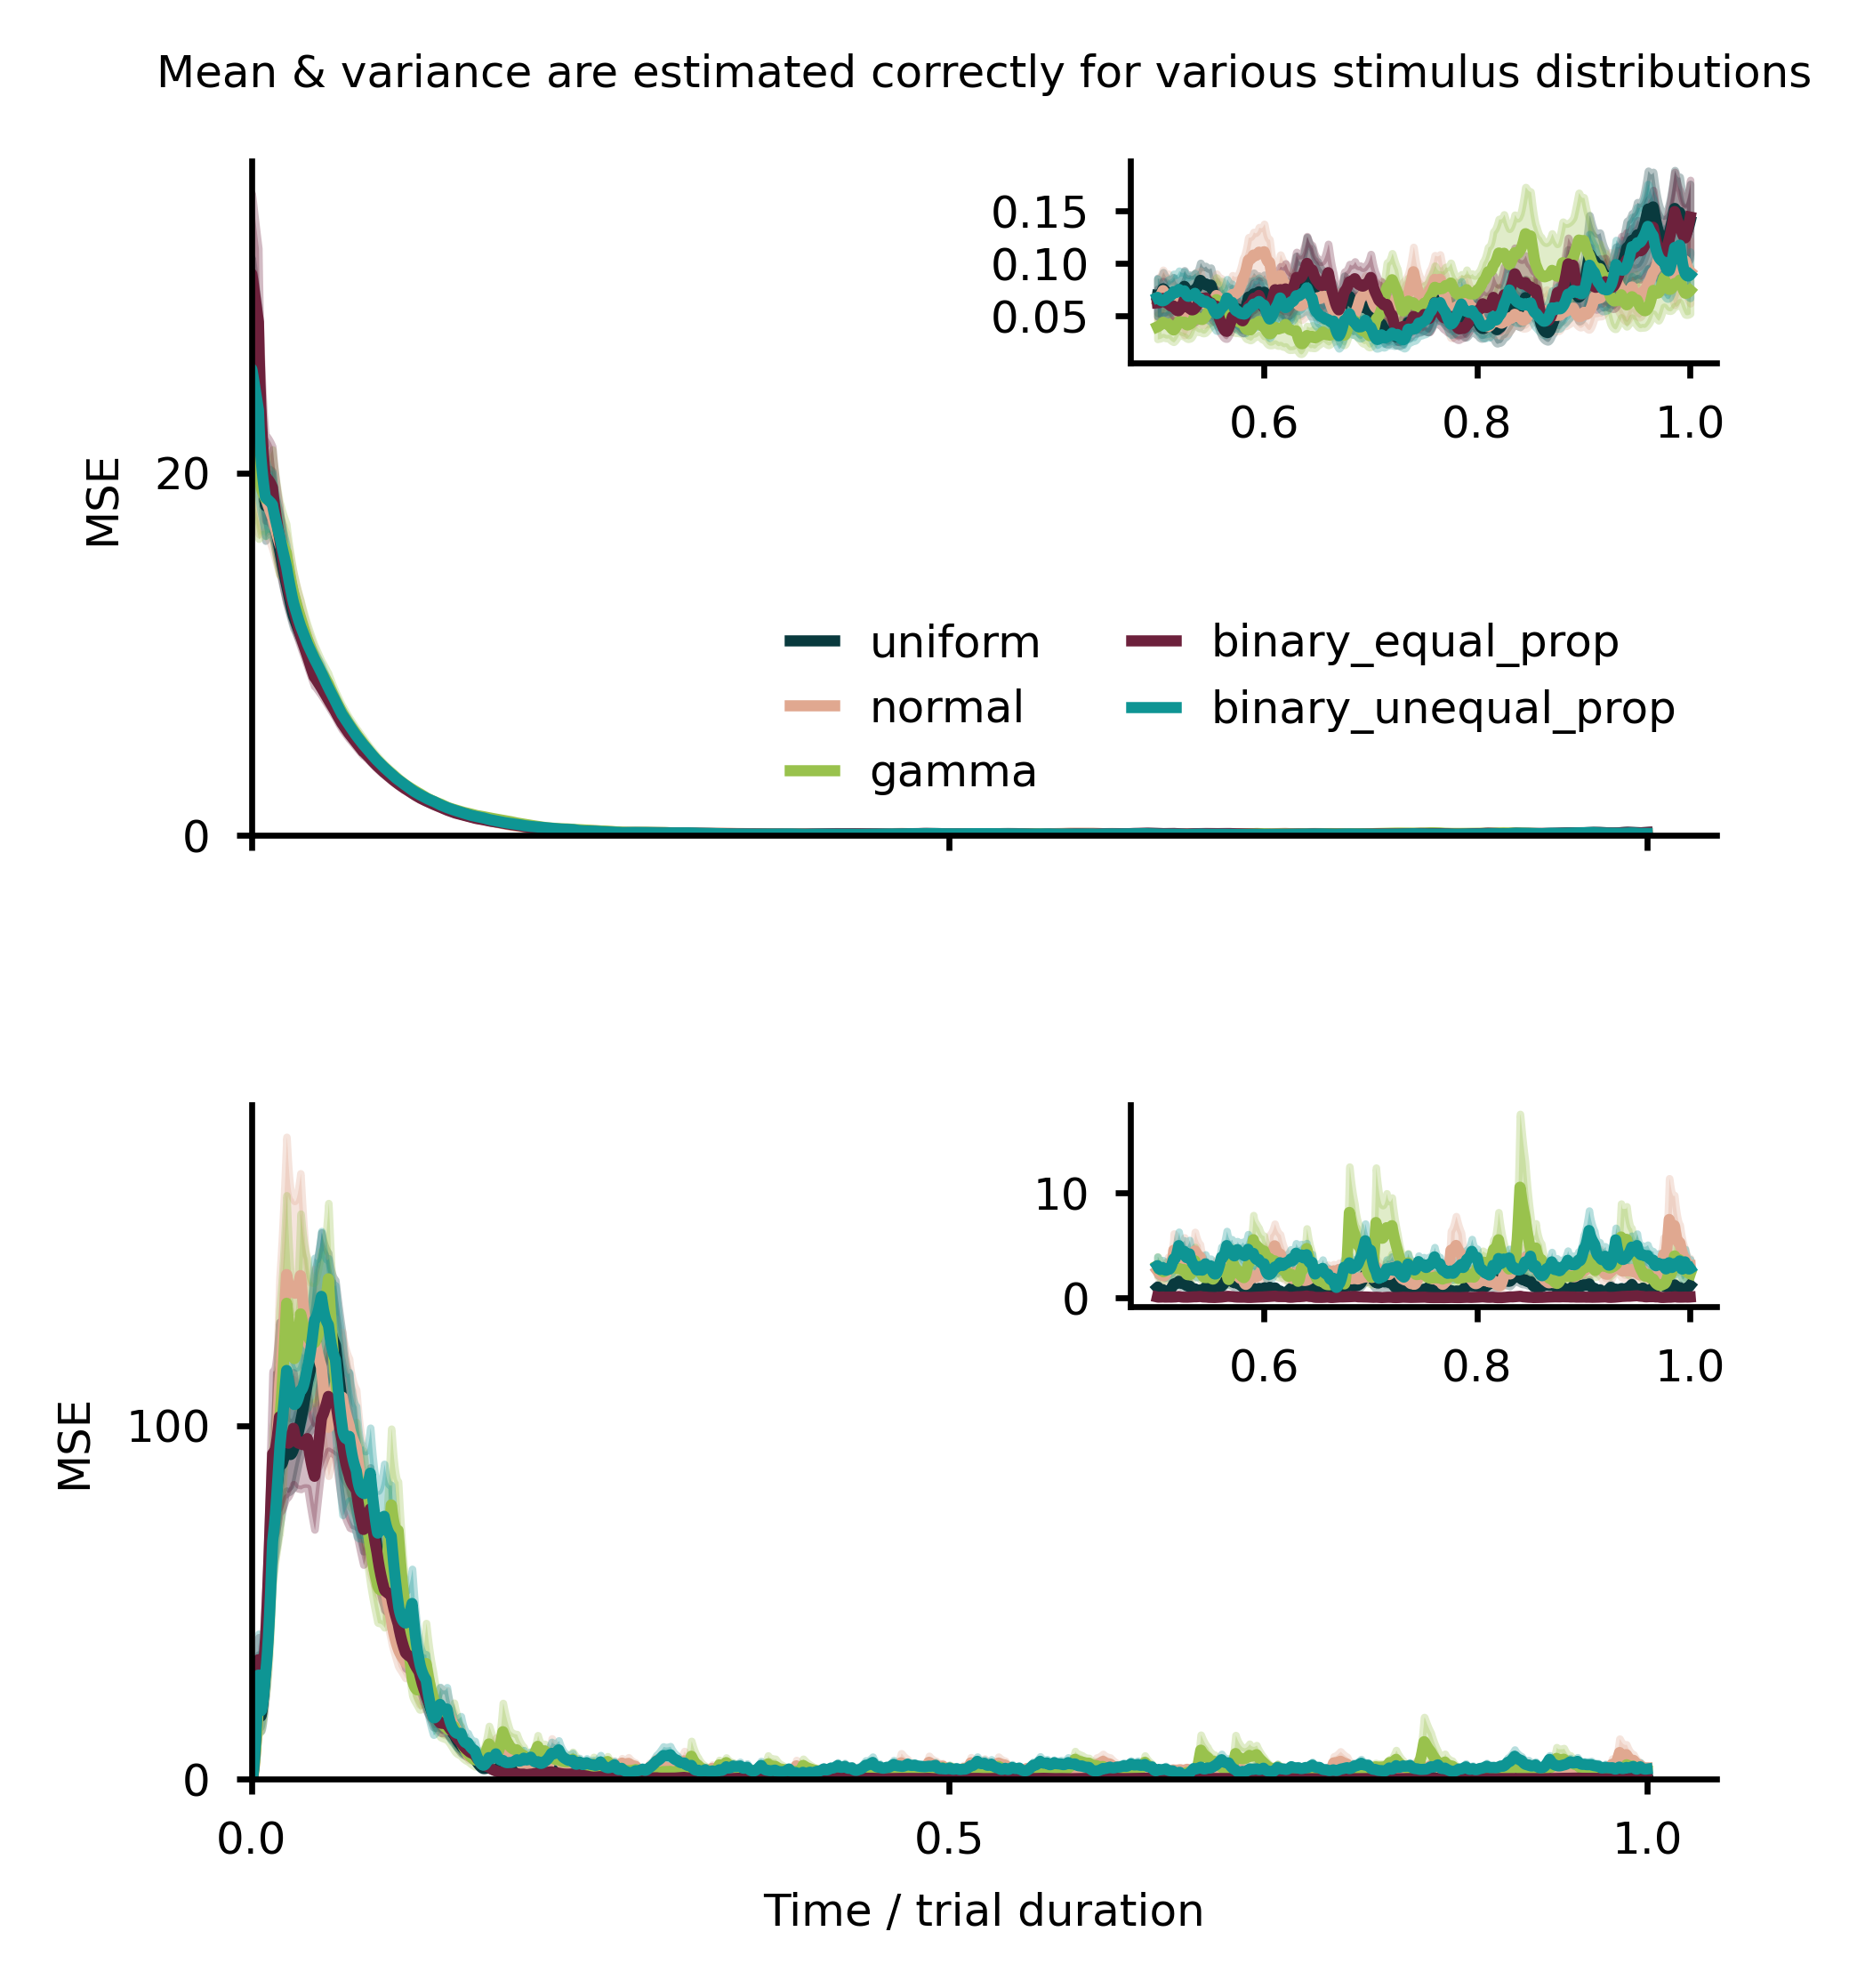
\includegraphics[scale=1]{../results/figures/final/Fig_2_S1}% [width=1\linewidth]
\caption{\footnotesize{\bf Estimation of mean and variance for different stimulus distributions.\newline}  
Top: The mean-squared error (MSE) between the running average and the activity of the M neuron decreases to a near-zero level for all stimulus distributions tested. 
Bottom: The MSE between the instantaneous variance and the V neuron decreases to a low level with minor differences between the distributions tested. Zoom-in shows the last half of the trial. Mean of the stimulus distribution = XXX, Variance of the stimulus distribution = XXX.
}
\label{fig:Fig_2_S1}
\end{figure}


\begin{figure}[!h]
	\centering
    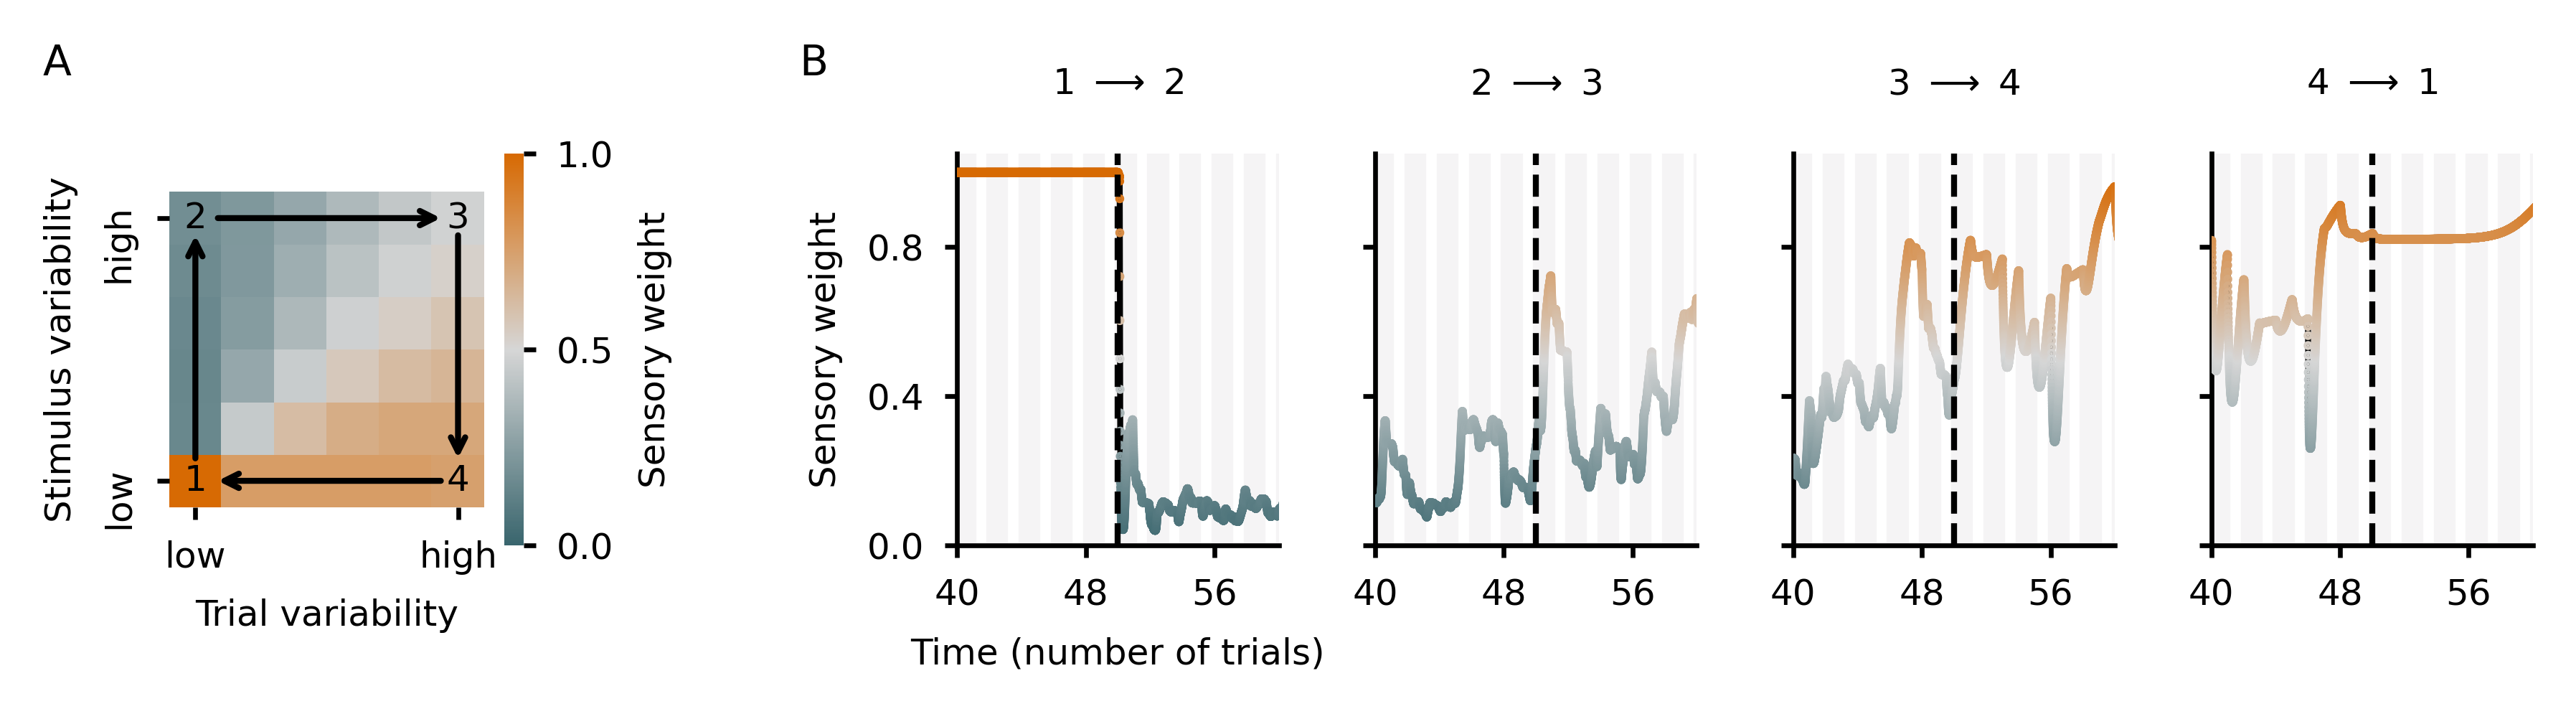
\includegraphics{../results/figures/final/Fig_3_S1}% [width=1\linewidth]
\caption{\footnotesize{\bf Dynamic variance estimation allows flexible adaptation to changes in the stimulus statistics and environment. \newline}  
{\bf (A)} Sensory weight for different input statistics (same as in Fig. \ref{fig:Fig_3}E). Numbers denote specific example states. Arrows denote the transitions between those states.
{\bf (B)} The sensory weight over time is shown for all transitions in (A). The switch to a new input statistics occurs at trial 60. Parameters are taken from Fig. \ref{fig:Fig_3}.
}
\label{fig:Fig_3_S1}
\end{figure}


\begin{figure}[!h]
	\centering
    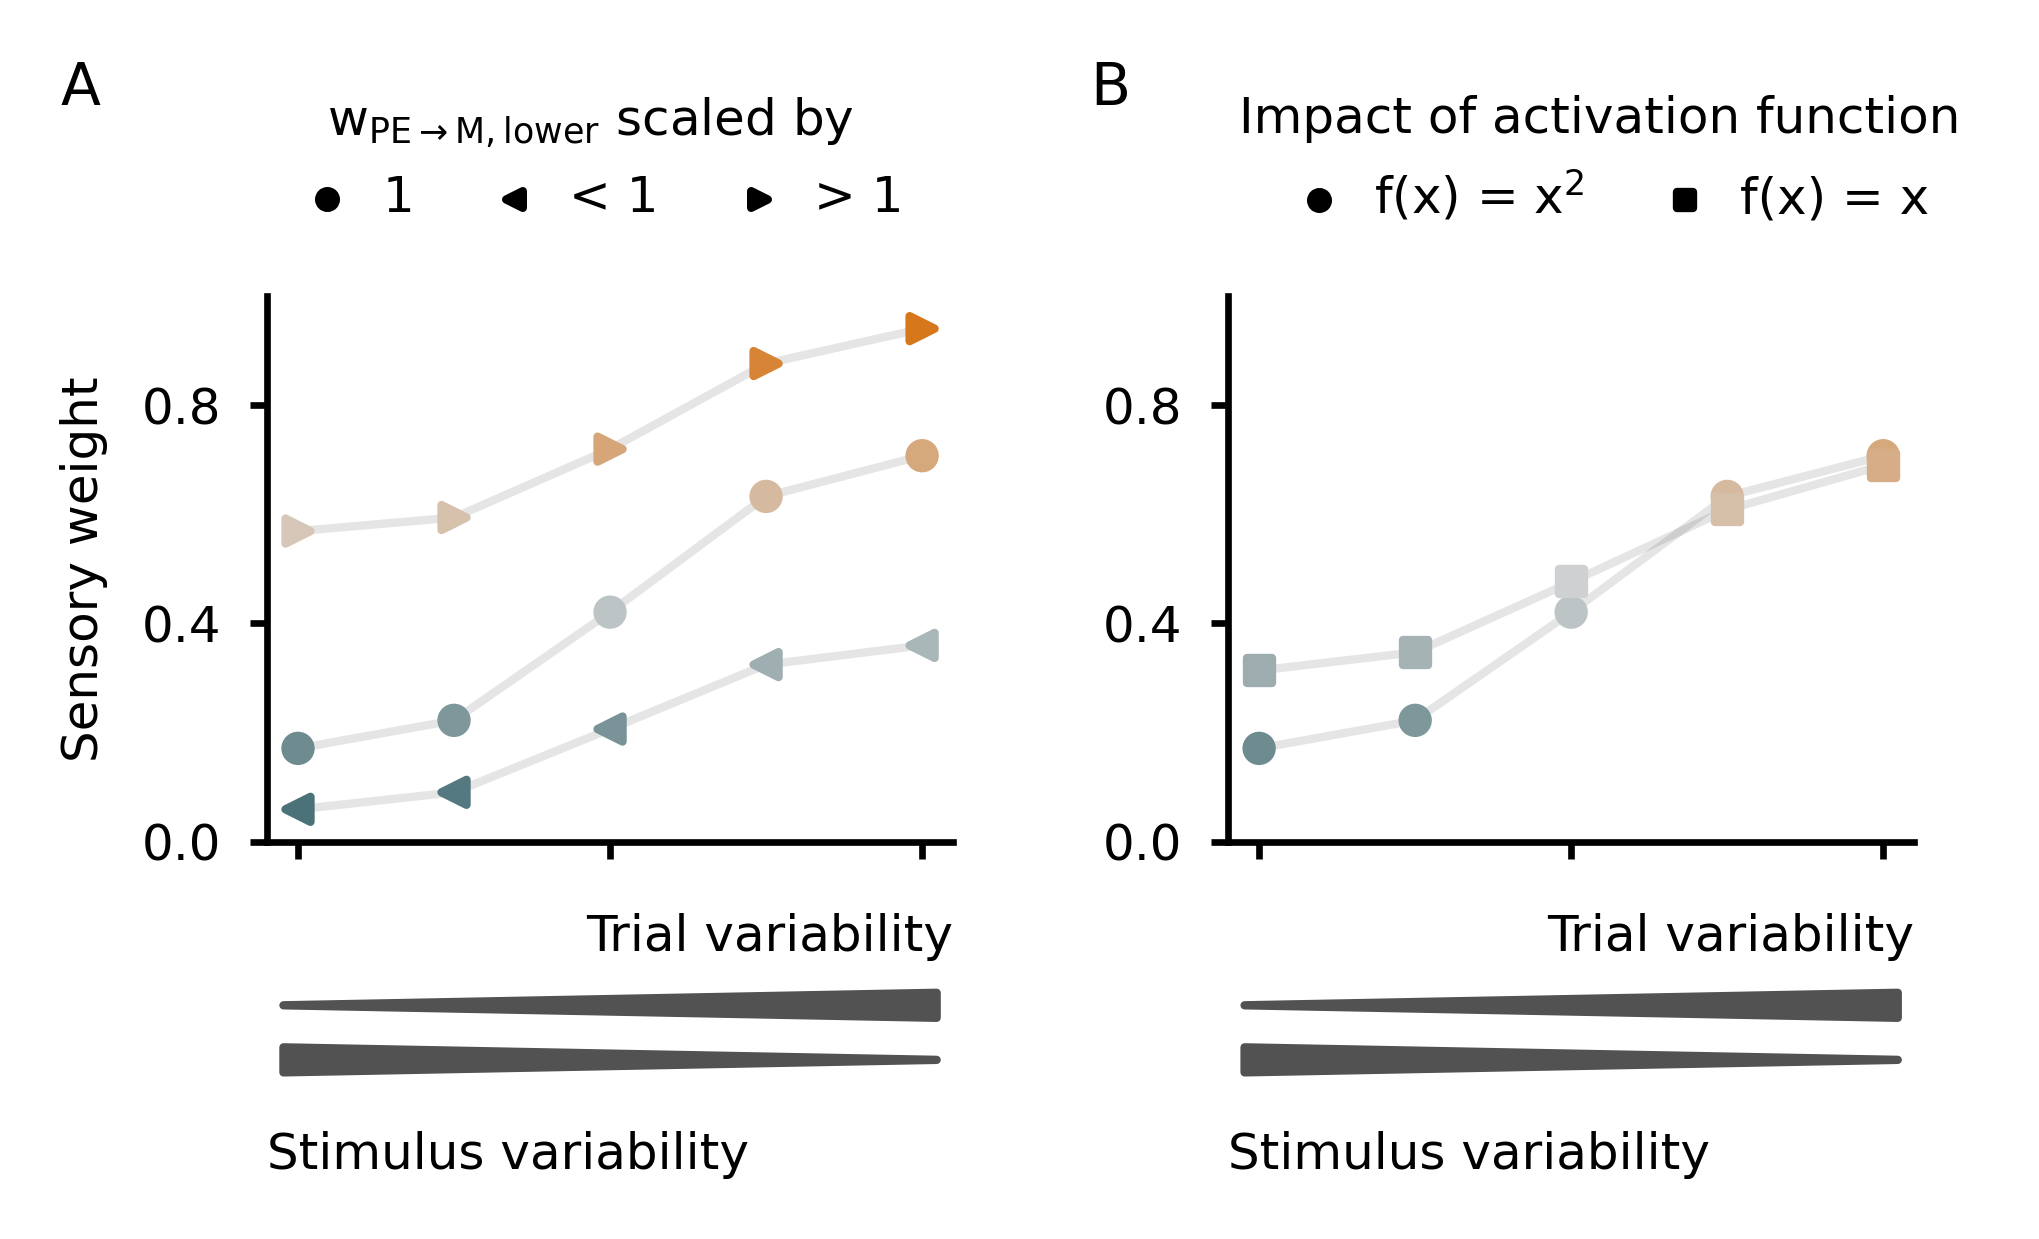
\includegraphics{../results/figures/final/Fig_3_S2}% [width=1\linewidth]
\caption{\footnotesize{\bf Perturbing the weighting of sensory inputs and predictions by altering  network properties. \newline}  
{\bf (A)} The weights from the lower-level PE neurons to the M neuron are scaled by a factor below 1 (here, xxx) or above 1 (here, xxx), leading to a distorted weighting. If the update of the M neuron in the lower subnetwork is too slow ($\blacktriangleleft$), the prediction is overrated. If the update of the M neuron in the lower subnetwork is too fast ($\blacktriangleright$), the sensory input is overrated.
{\bf (B)} The precise activation function for the V neurons does not have a major impact on the sensory weight. Only for inputs with high stimulus variability, the sensory stimulus is slightly overrated when the squared activation function is replaced by a linear, rectified activation function.
}
\label{fig:Fig_3_S2}
\end{figure}


\begin{figure}[!h]
	\centering
    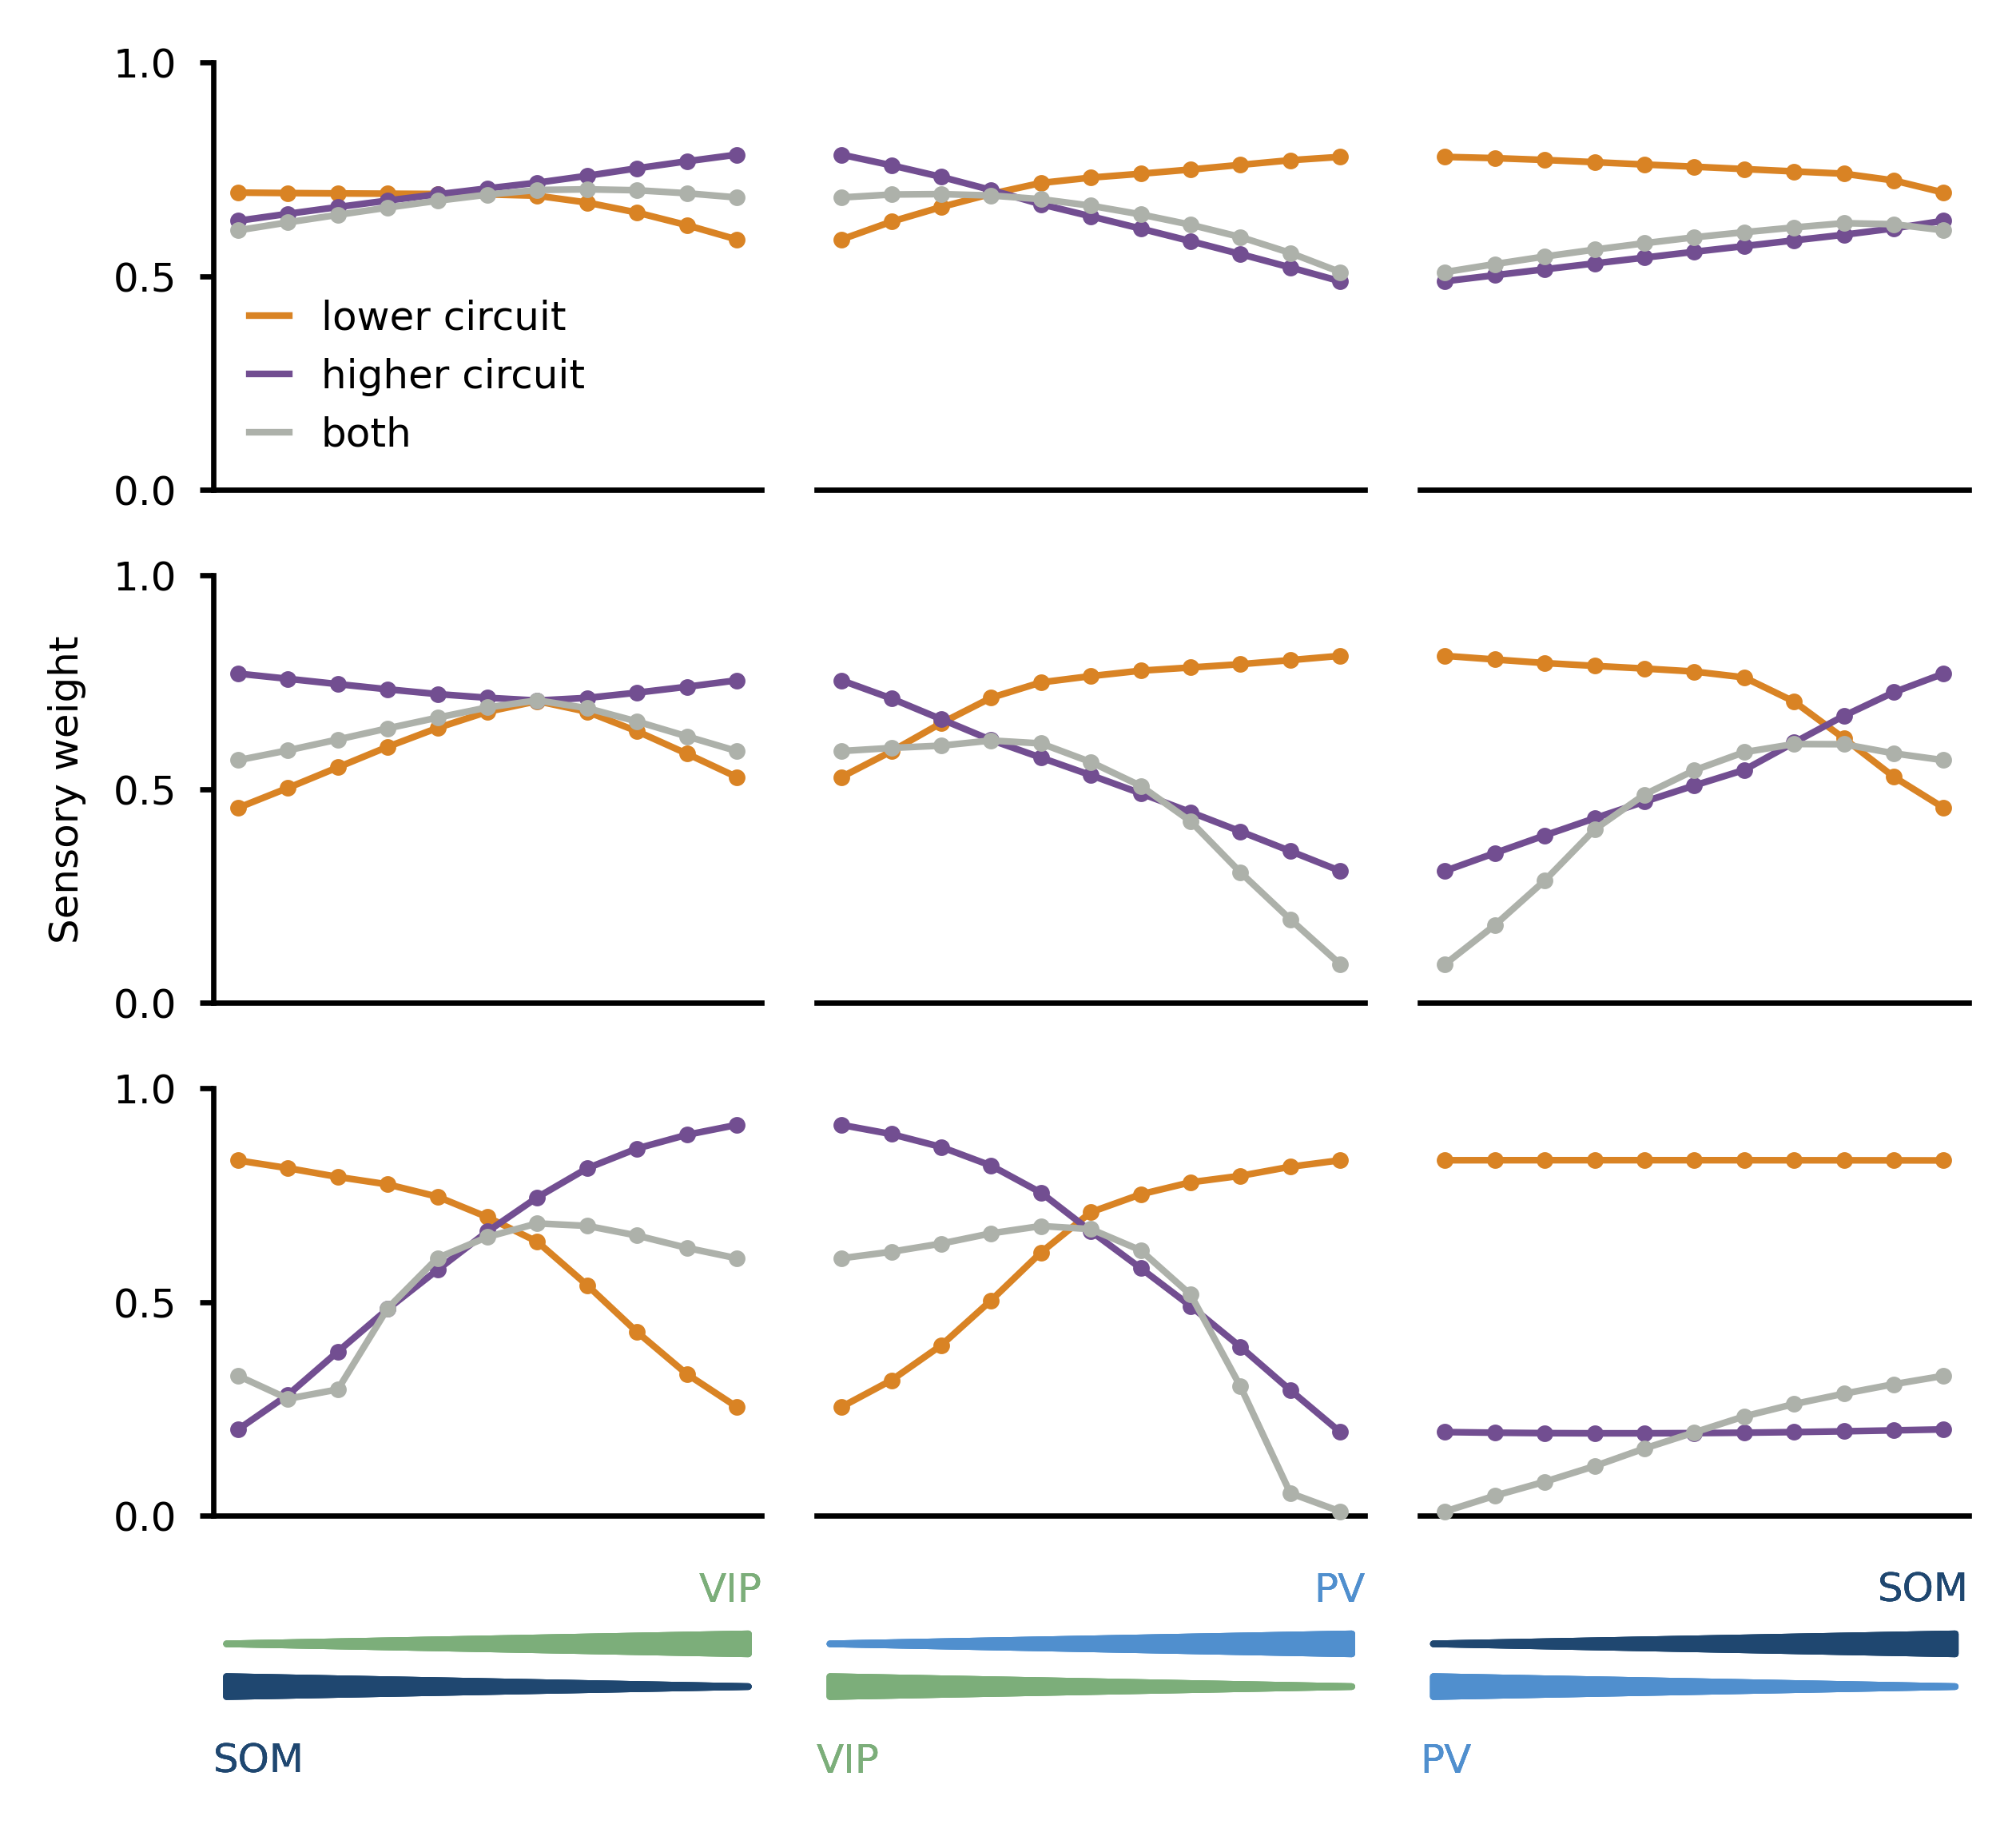
\includegraphics{../results/figures/final/Fig_4_S1}% [width=1\linewidth]
\caption{\footnotesize{\bf Neuromodulators acting locally either on interneurons in the lower or higher PE circuit. \newline}  
{\bf (A)} Sensory weight changes with neuromodulators acting on interneurons in the lower PE circuit.
{\bf (B)} Sensory weight changes with neuromodulators acting on interneurons in the lower PE circuit. Simulation parameters, labels and colors as in Fig. \ref{fig:Fig_4}. 
}
\label{fig:Fig_4_S1}
\end{figure}


\begin{figure}[!h]
	\centering
    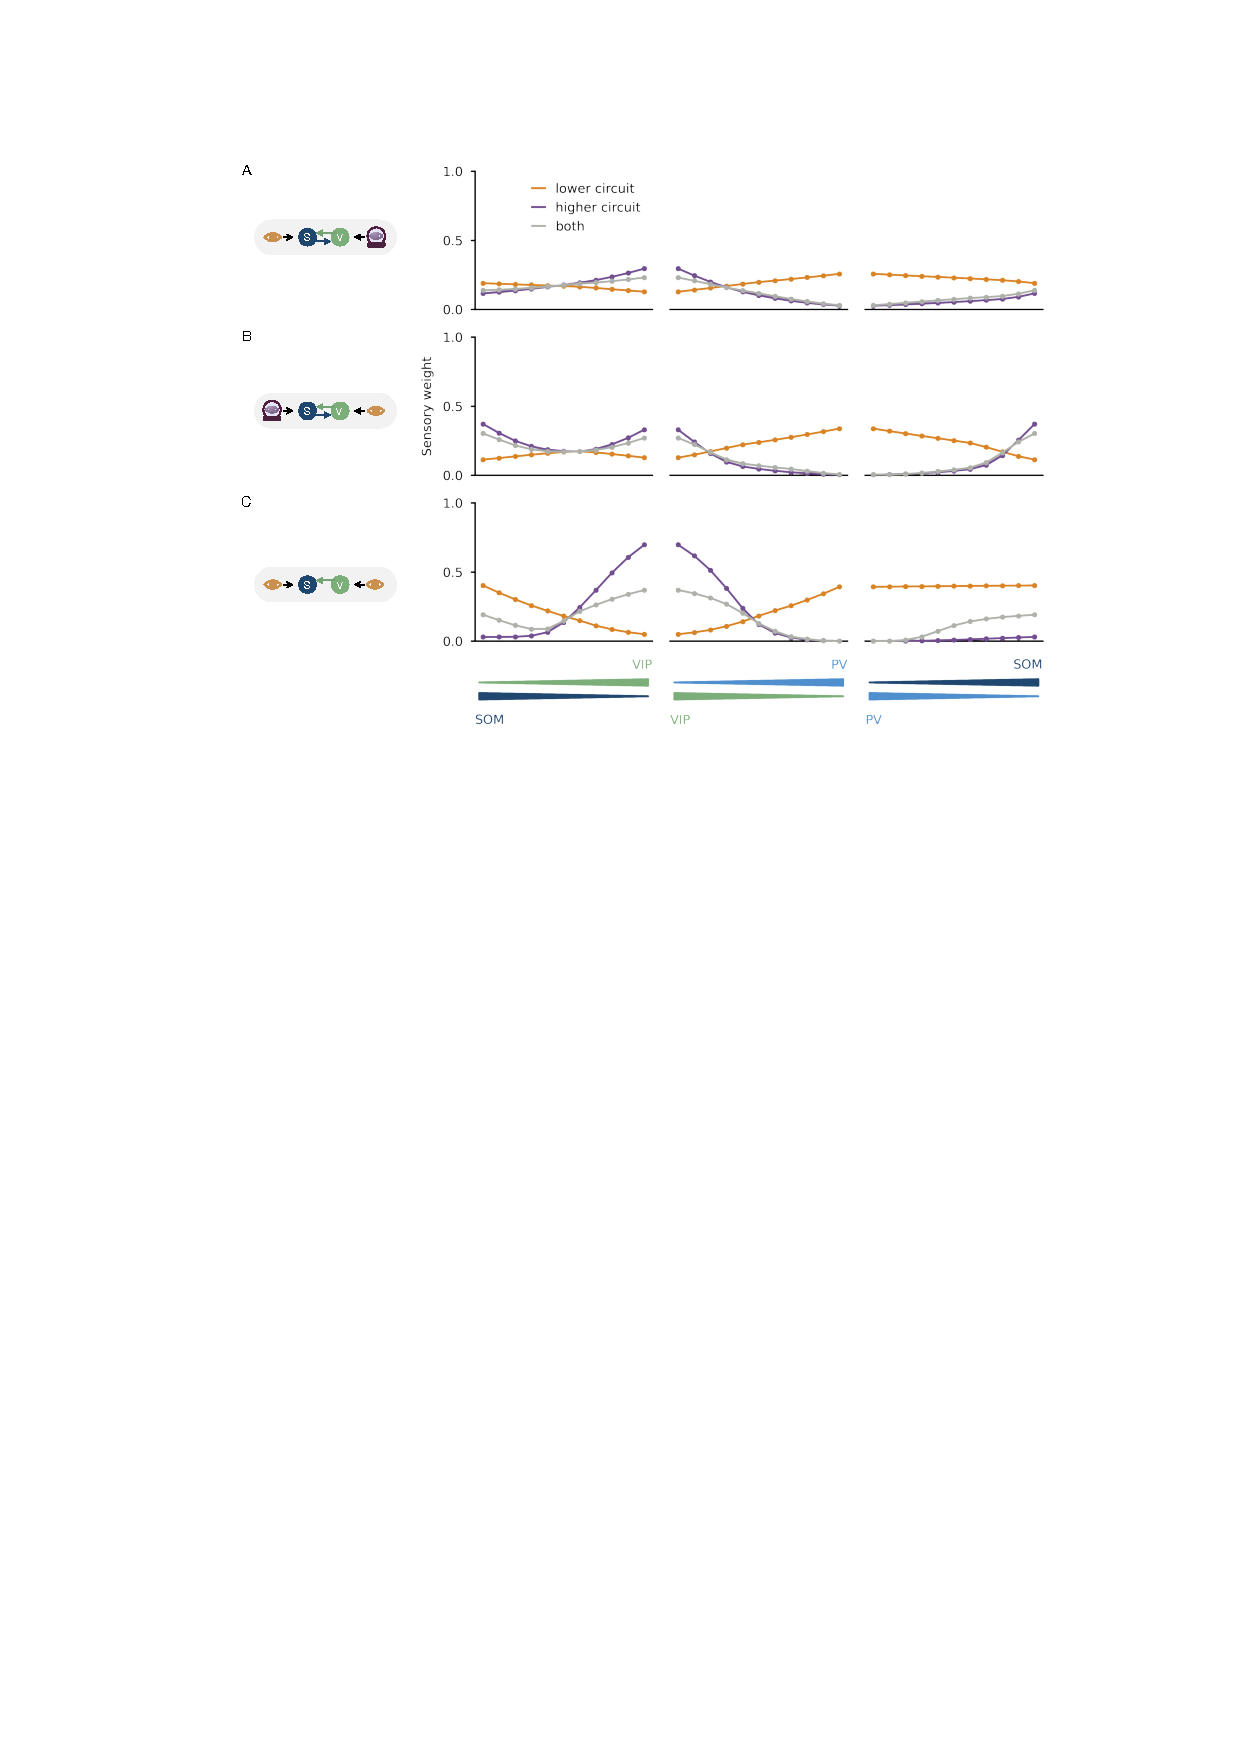
\includegraphics{../results/figures/final/Fig_4_S2}% [width=1\linewidth]
\caption{\footnotesize{\bf Perturbing the interneurons changes the baseline and gain of nPE and pPE neurons.\newline}  
{\bf (A)} Changes in the baseline activity of nPE and pPE neurons for different interneurons targeted. 3 different mean-field networks are tested.
{\bf (B)} Same as in (A) but for the gain of nPE and pPE neurons. Simulation parameters, labels, and colors as in Fig. \ref{fig:Fig_4}. 
}
\label{fig:Fig_4_S2}
\end{figure}


\end{document}
